\newcommand{\nn}{\nonumber}
\newcommand{\vpi}{\mathbf \pi}
\newcommand{\vecd}{\mathbf d}
\newcommand{\matC}{\mathbf C}
\newcommand{\matQ}{\mathbf Q}

\newcommand{\om}{\Omega_\mr m}
\newcommand{\omb}{\Omega_\mr b}
\newcommand{\sig}{\sigma_8}
\newcommand{\ns}{n_s}
\newcommand{\w}{w_0}
\newcommand{\wa}{w_a}

\renewcommand{\d}{{\rm d}}
\newcommand{\pd}{P_{\delta}}
\newcommand{\pe}{P_\mr E}

\newcommand{\vt}{\vartheta}
\newcommand{\vp}{\varphi}
\newcommand{\eps}{\epsilon}
\newcommand{\abs}[1]{| #1 |}
\newcommand{\mr}{\mathrm}

\renewcommand{\d}{{\rm d}}

\newcommand{\like}{L}
\newcommand{\prob}{P}
\newcommand{\probr}{P_r}
\newcommand{\p}{\mathbf p}
\newcommand{\pco}{\mathbf p_\mr{c}}
\newcommand{\pnu}{\mathbf p_\mr{n}}
\newcommand{\plf}{\mathbf p_\mr{LF}}
\newcommand{\D}{\mathbf D}
\newcommand{\Del}{\mathbf \Delta}
\newcommand{\M}{\mathbf M}
\newcommand{\N}{\mathbf N}
\newcommand{\U}{\mathbf U}


\begin{summary}
We developed a unique and coherent cosmological forecast software package, \CoLi. Using this single unified framework, we revised the HLSS and HLIS cosmological forecasts, including systematics effects. We also pioneered a joint HLSS-HLIS analysis. This led us to emphasize the importance and the power of a \emph{multi-probe} cosmological approach. We also performed several trade studies to support Project Office activities, in conjunction with the SNe SITs.
\end{summary}


In this section we will describe the results a simulated likelihood analysis that forecasts science return and quantified systematics for different choices in the WFIRST HLS survey. We first introduce the \CoLi software framework that was used to generate our forecasts. We then present forecasts for HLSS and HLIS specific observables. We conclude with a summary of ongoing research to explore WFIRST multi-probe analysis strategies, i.e., to combine all WFIRST observables and their correlated systematics consistently in simulated likelihood analyses. We also present ongoing work that will assess synergies between WFIRST and other contemporary surveys, e.g., the ground-based, optical Large Synoptic Survey Telescope (LSST) and future missions studying the Cosmic Microwave Background, e.g. CMB-Stage4 (CMB-S4) experiments.

\subsection{\CoLi Introduction}
\label{sec:cosmolike}

\begin{summaryii}
  \CoLi is unique in its approach that jointly models LSS probes as well as their correlated systematics. It is the only code that computes multi-probe covariances, including the (dominant) higher-order terms of the matter density field.
\end{summaryii}

\CoLi has been used in several science efforts, e.g. the combined probes forecasts presented in \citep{Eifler:2014}, an analysis of SDSS shear data \citep{Huff2014}, and efforts to develop new mitigation strategies for baryonic physics \citep{Eifler2015} and galaxy intrinsic alignment \citep{Krause2016}. It is one of two cosmology analysis pipelines used by the ongoing Dark Energy Survey's Year 1 analysis and it has previously been used in the DES science verification data analysis \citep{DES2015}. Beyond DES,
%===
\begin{figure}
  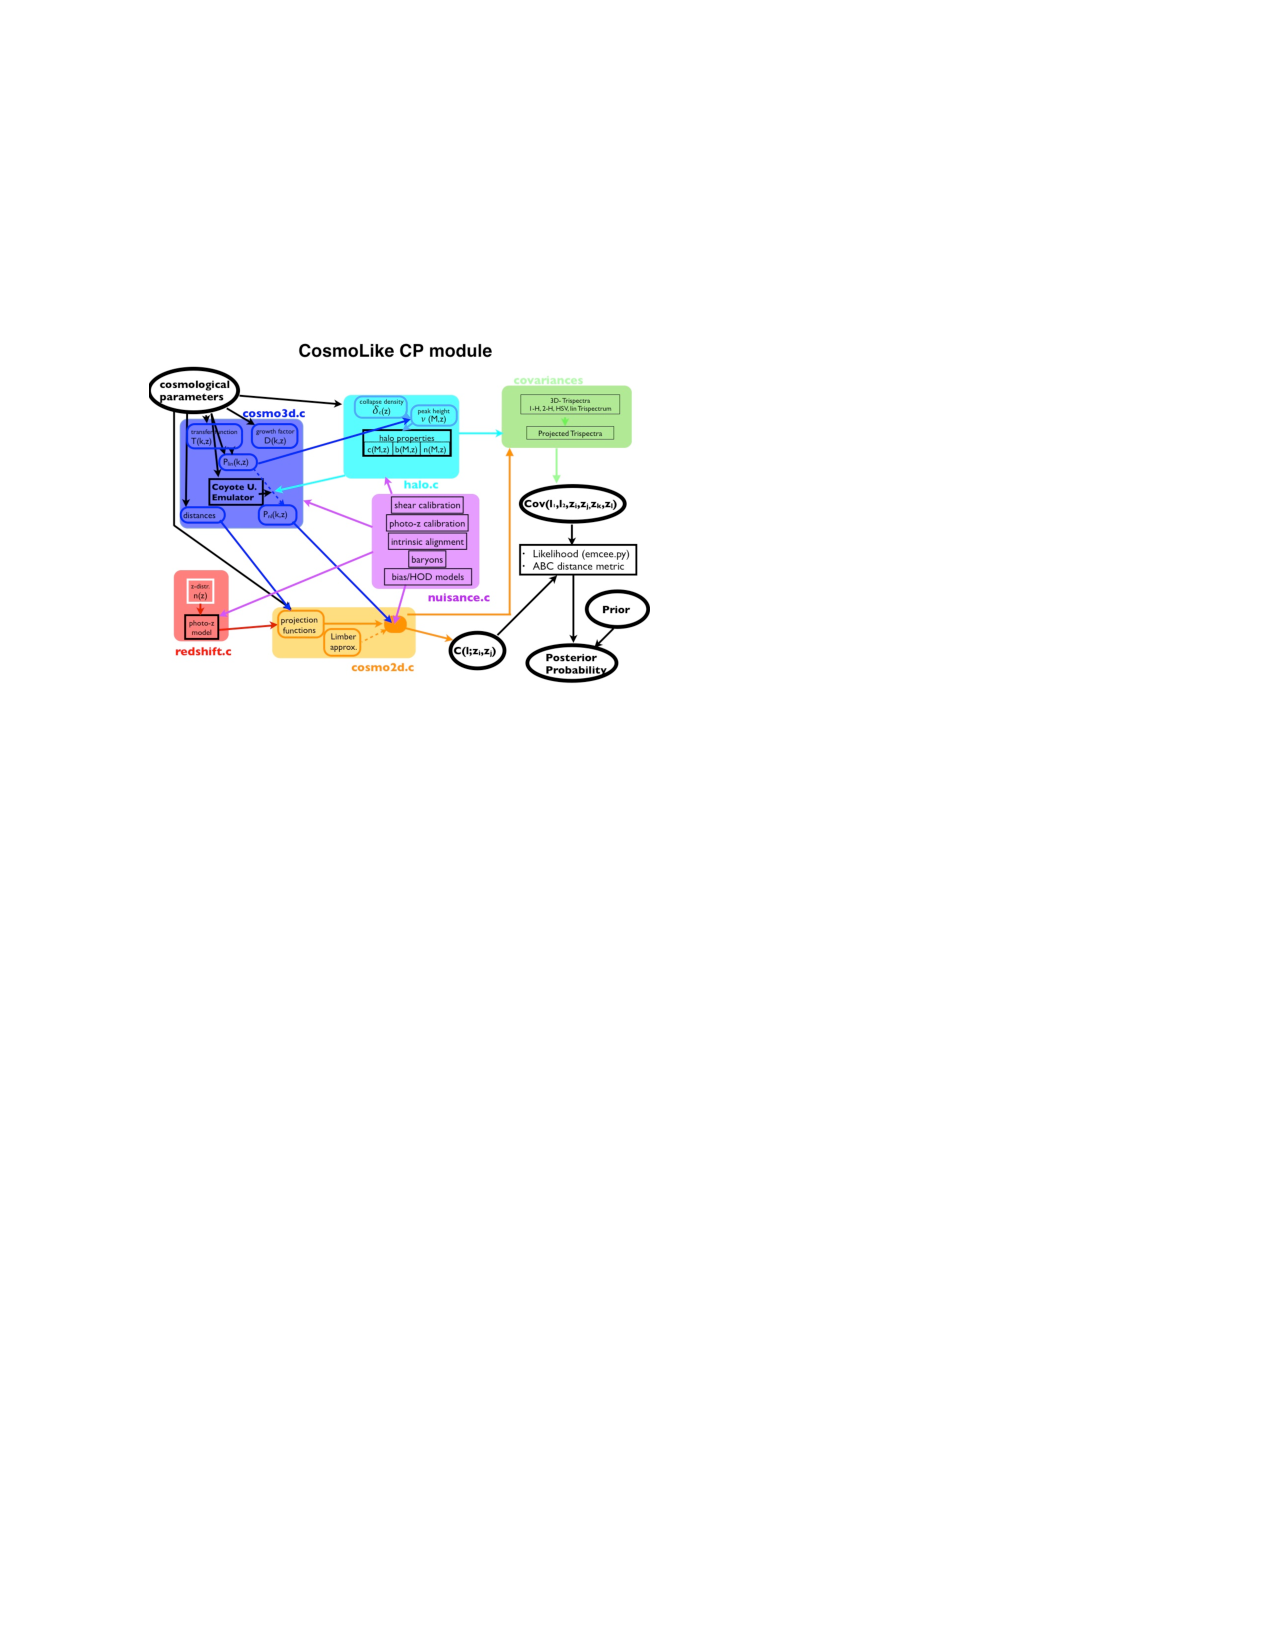
\includegraphics[width=16.0cm]{Plots/forecasts/cosmolike_codestruct}
   \caption{Illustration of a subset of CosmoLike's code structure. Starting from cosmological parameters we show how different parts of the code interface and how projected summary statistics for various observables are obtained. This particular workflow corresponds to the multi-probe analysis as described in Sect. {\ref{sec:multi-probe}}. For the HLSS survey a subset of these routines are being used.
}
  \label{fi:fcosmolike}
\end{figure}
%===
the code has been used to simulate a realistic multi-probe likelihood analyses for LSST \citep{Krause2017} that include cosmic shear, galaxy clustering, galaxy-galaxy lensing, cluster number counts and cluster weak lensing.
The software relies on a massively parallelized computation of fine-tuned look-up tables with a targeted sub-second run-time per point in parameter space. Given the large number of parameters describing systematic effects in future LSS analyses, this efficient computation ensures an acceptable turnaround time for analyses. In particular, it allows one to generate a large number of simulated likelihood analyses which is necessary to optimize future surveys. Figure~\ref{fi:fcosmolike}
illustrates the \CoLi combined probes module we plan to use for the proposed analysis. Starting from a cosmological model, this schematic illustrates how projected power spectra for various LSS probes are computed:
\begin{enumerate}
\item In the first step \CoLi computes the 3D-density power spectrum using one of 3 different methods. The density power spectrum can be modeled using the latest suites of numerical simulations, i.e. the Coyote Universe emulator \citep{Heitmann2014}, or the latest implementation of Halofit \citep{tsn12}, or using a state-of-the-art analytic halo model \citep{Krause2013}.
\item Given a survey specific redshift distribution \CoLi computes projected (tomographic) 2D power spectra for WL, galaxy-galaxy lensing, and galaxy clustering.
\item  For galaxy-galaxy lensing and galaxy clustering, the connection between dark and luminous matter is modeled using either a linear bias model or a sophisticated (but computationally slower) HOD model \citep{Krause2013}.
\item The covariance is computed analytically using perturbation theory to include the higher-order moments of the density field, including the Halo Sample Variance contribution that dominates the statistical error budget. This covariance takes all cross-correlations between the different probes into account.
\item \CoLi has various systematics modeling capabilities, in particular it can account for baryonic effects, intrinsic alignment, shear calibration and photo-z uncertainties \citep{Eifler2015, Krause2016, Krause2017}.
\item If one chooses to use two-point correlation functions instead of power spectra CosmoLike offers an extremely fast Fourier transformation using a Hankel transform. The code employs a parallel MCMC sampling technique \citep{Goodman2010}, implemented using the emcee python package \citep{Foreman-Mackey2013}.
\end{enumerate}


\subsection{HLS Spectroscopic Survey Forecasts and Trade Studies}

\begin{summaryii}
  We implemented in the \CoLi package a state of the art spectroscopic survey forecasting formalism. We used this tool to update the HLSS forecast and to conduct two trade studies. We validated and explored the validity of science requirements HLSS1 and HLSS3. (\S~\ref{sec:sr2a_grs}).
  \begin{enumerate}
  \item We carried out a trade study of area versus depth for the HLSS only, starting from a baseline survey of 2,227 sq. deg. and a wavelength range of 1.05-1.85 microns. We considered two alternative scenarios, i.e., a survey twice as wide and a survey half as wide but correspondingly deeper.
  \item We examined the impact of an extended wavelength range on the cosmological constraining power.
\end{enumerate}
\end{summaryii}

\subsubsection{Varying the HLSS Area} The galaxy redshift distributions were computed using the WFIRST \texttt{Exposure Time Calculator ETC v14}. The H$\alpha$ forecasts are based on the
average of the 3 models in \citet{Pozzetti:2016}, and the [O III] forecasts are
based on the \citet{Mehta:2015} luminosity function. The resulting redshift
distributions are displayed in Figure~\ref{fi:forecast1} (left panel). We extended the \CoLi framework \citep{Eifler:2014,Krause2017} to compute the constraining power of all cosmic acceleration scenarios, closely following \citet{Wang2013}. We ran a
500,000 step MCMC simulated likelihood analysis in a 23 dimensional parameter
space. We simultaneously varied 7 cosmological parameters and 16 nuisance
parameters describing uncertainties due to the linear galaxy bias model, the
non-linear smearing of the BAO feature, peculiar velocity dispersion, power
spectrum shot noise, and redshift errors. We assumed priors on cosmological
parameters from the current state of the art experiments, i.e. the Planck
mission, the Baryon Oscillation Spectroscopic Survey, the Joint Lightcurve
Analysis, as described in \citet{Aubourg:2015}.

The information gain is quantified using the standard Dark Energy Task Force FOM and an extended cosmology FOM, which measures the enclosed volume in the full 7-dimensional cosmological parameter space, not just in the 2 dark energy parameters. We will refer to these FOMs as DE-FOM and Cosmo-FOM. Compared to our baseline scenario we find a decreased DE-FOM of 32\% and a decreased Cosmo-FOM of 45\% for the shallow/large area survey. For the deep/small area survey we find an increased DE-FOM of 5\% and an increased Cosmo-FOM of 2\%. We note that these findings are model and prior dependent and recommend further studies to confirm these forecasts. We also note that the [O III] numbers are pending a future update in part due to the reduction in the baseline telescope temperature to 260 K.
\begin{figure*}
  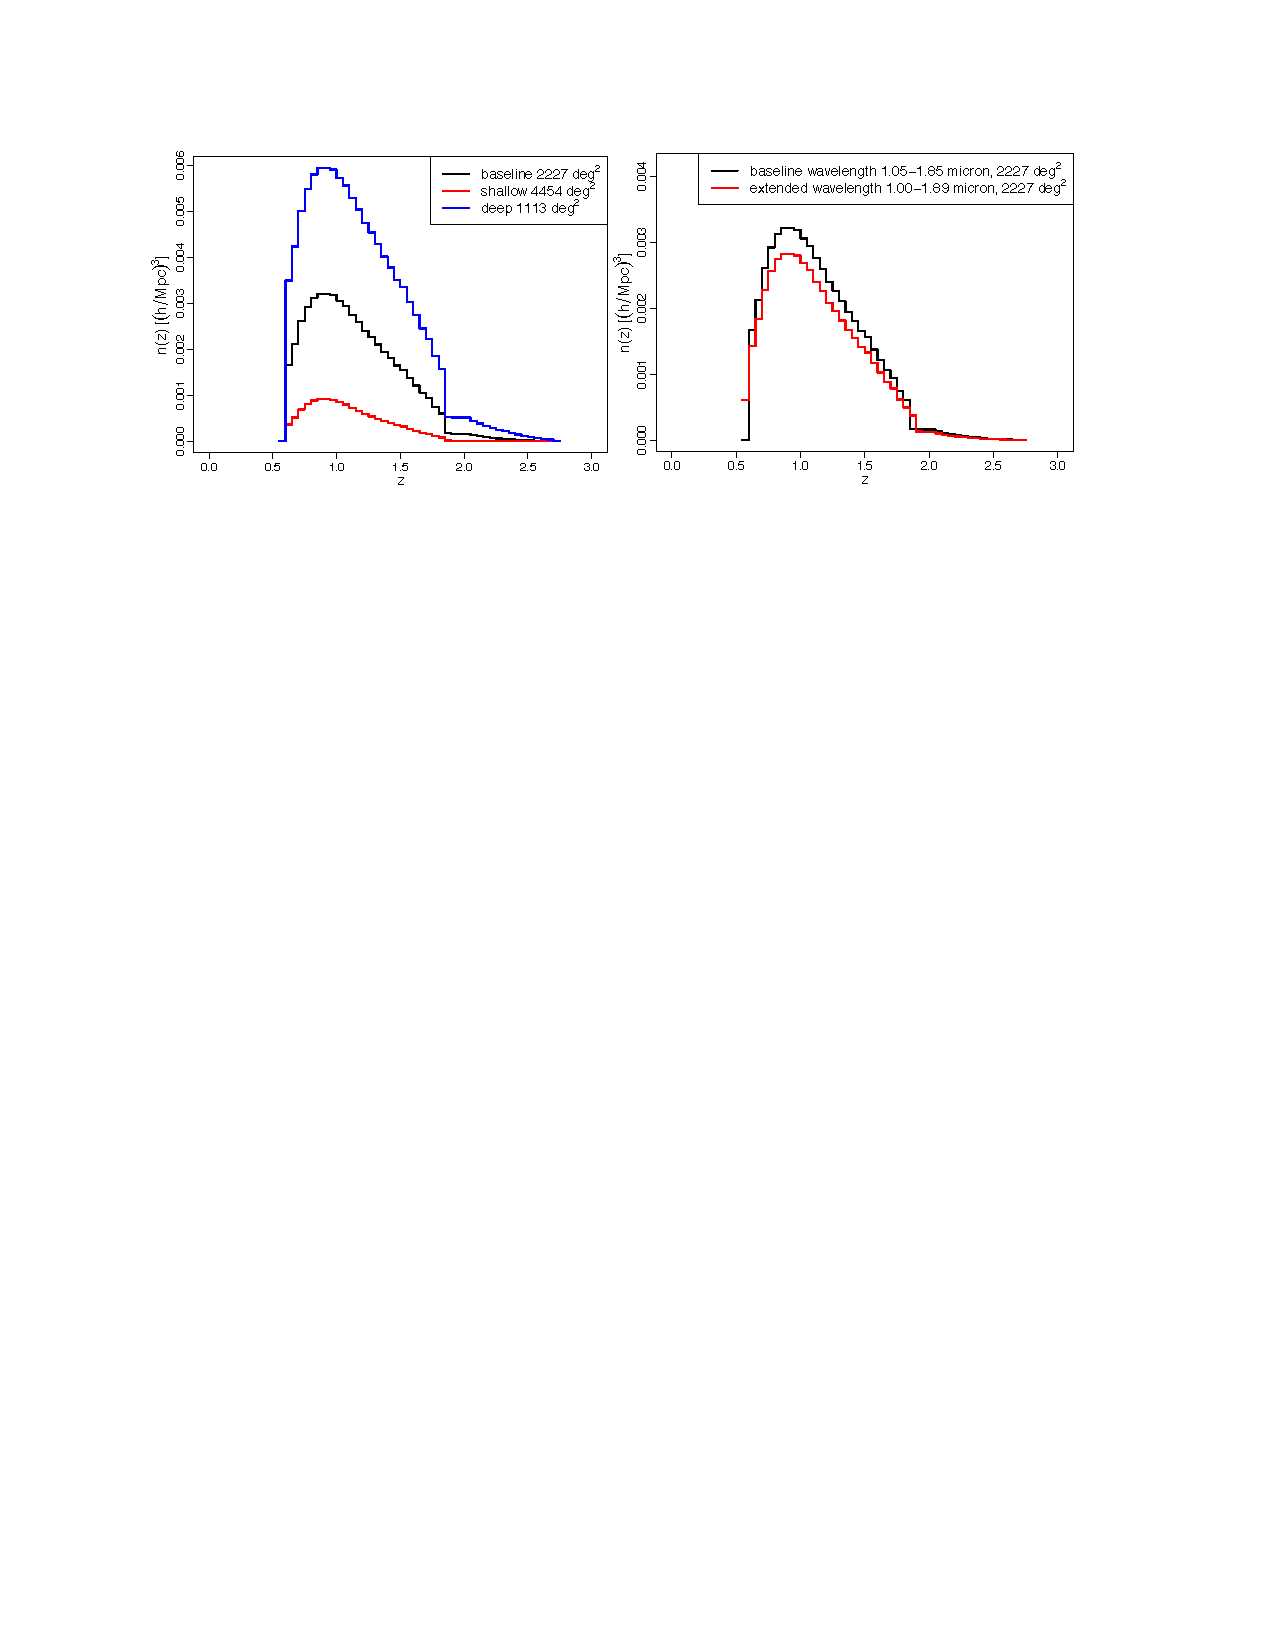
\includegraphics[width=16.0cm]{Plots/forecasts/HLSS_forecasts}
    \caption{\textit{Left:}Redshift distribution of galaxies in the baseline, the shallow/large area, and the deep/small area survey. \textit{Right:} Redshift distribution of galaxies in the baseline and extended wavelength survey.
}
  \label{fi:forecast1}
\end{figure*}

%HLSS 3: The redshift range of galaxies surveyed shall encompass 1. $\leq$ z $\leq$ 2.7

\subsubsection{Varying the HLSS Redshift Coverage} In addition to the trade studies in HLSS 1 we examined the impact of an extended wavelength range on the DE-FOM and the Cosmo-FOM. We follow the same procedure as detailed in the HLSS 1 paragraph extending the wavelength range from 1.05-1.85 microns for the baseline model to 1.00-1.89 for the extended model. The corresponding redshift distributions of the galaxy samples computed from the ETC v1.14 are depicted in  Figure~\ref{fi:forecast1} (right panel). We find a decreased DE-FOM of 2\% and a decreased Cosmo-FOM of 11\% for the extended wavelength survey with respect to our baseline scenario. We iterate that these findings are model and prior dependent and recommend further studies varying the input parameters.

%%%%%%%%%%%%%%%%%%%%%%%%%%%%%%%%%%%
\subsection{HLS Imaging Survey Forecasts}
\label{sec:HLISforecasts}
%%%%%%%%%%%%%%%%%%%%%%%%%%%%%%%%%%%

\begin{summaryii}
We extended the \CoLi package to accurately forecast the HLIS weak gravitational lensing signal, including multiple additional systematics. This extension was then used to study multiple modifications to the survey and its requirements with a focus on the effect of systematics. In particular, we studied
\begin{enumerate}
  \item The science gain when extending the survey to 10,000 deg$^2$, instead if 2,200 deg$^2$;
  \item The combined impact of uncertainties in shape and photo-$z$ measurements;
  \item The impact of uncertainties in shape measurements only;
  \item The impact of uncertainties in photo-$z$ estimation only;
  \item The impact of uncertainties in baryonic physics modeling;
  \item The impact of uncertainties in intrinsic alignment modeling.
\end{enumerate}
\end{summaryii}

\begin{figure}
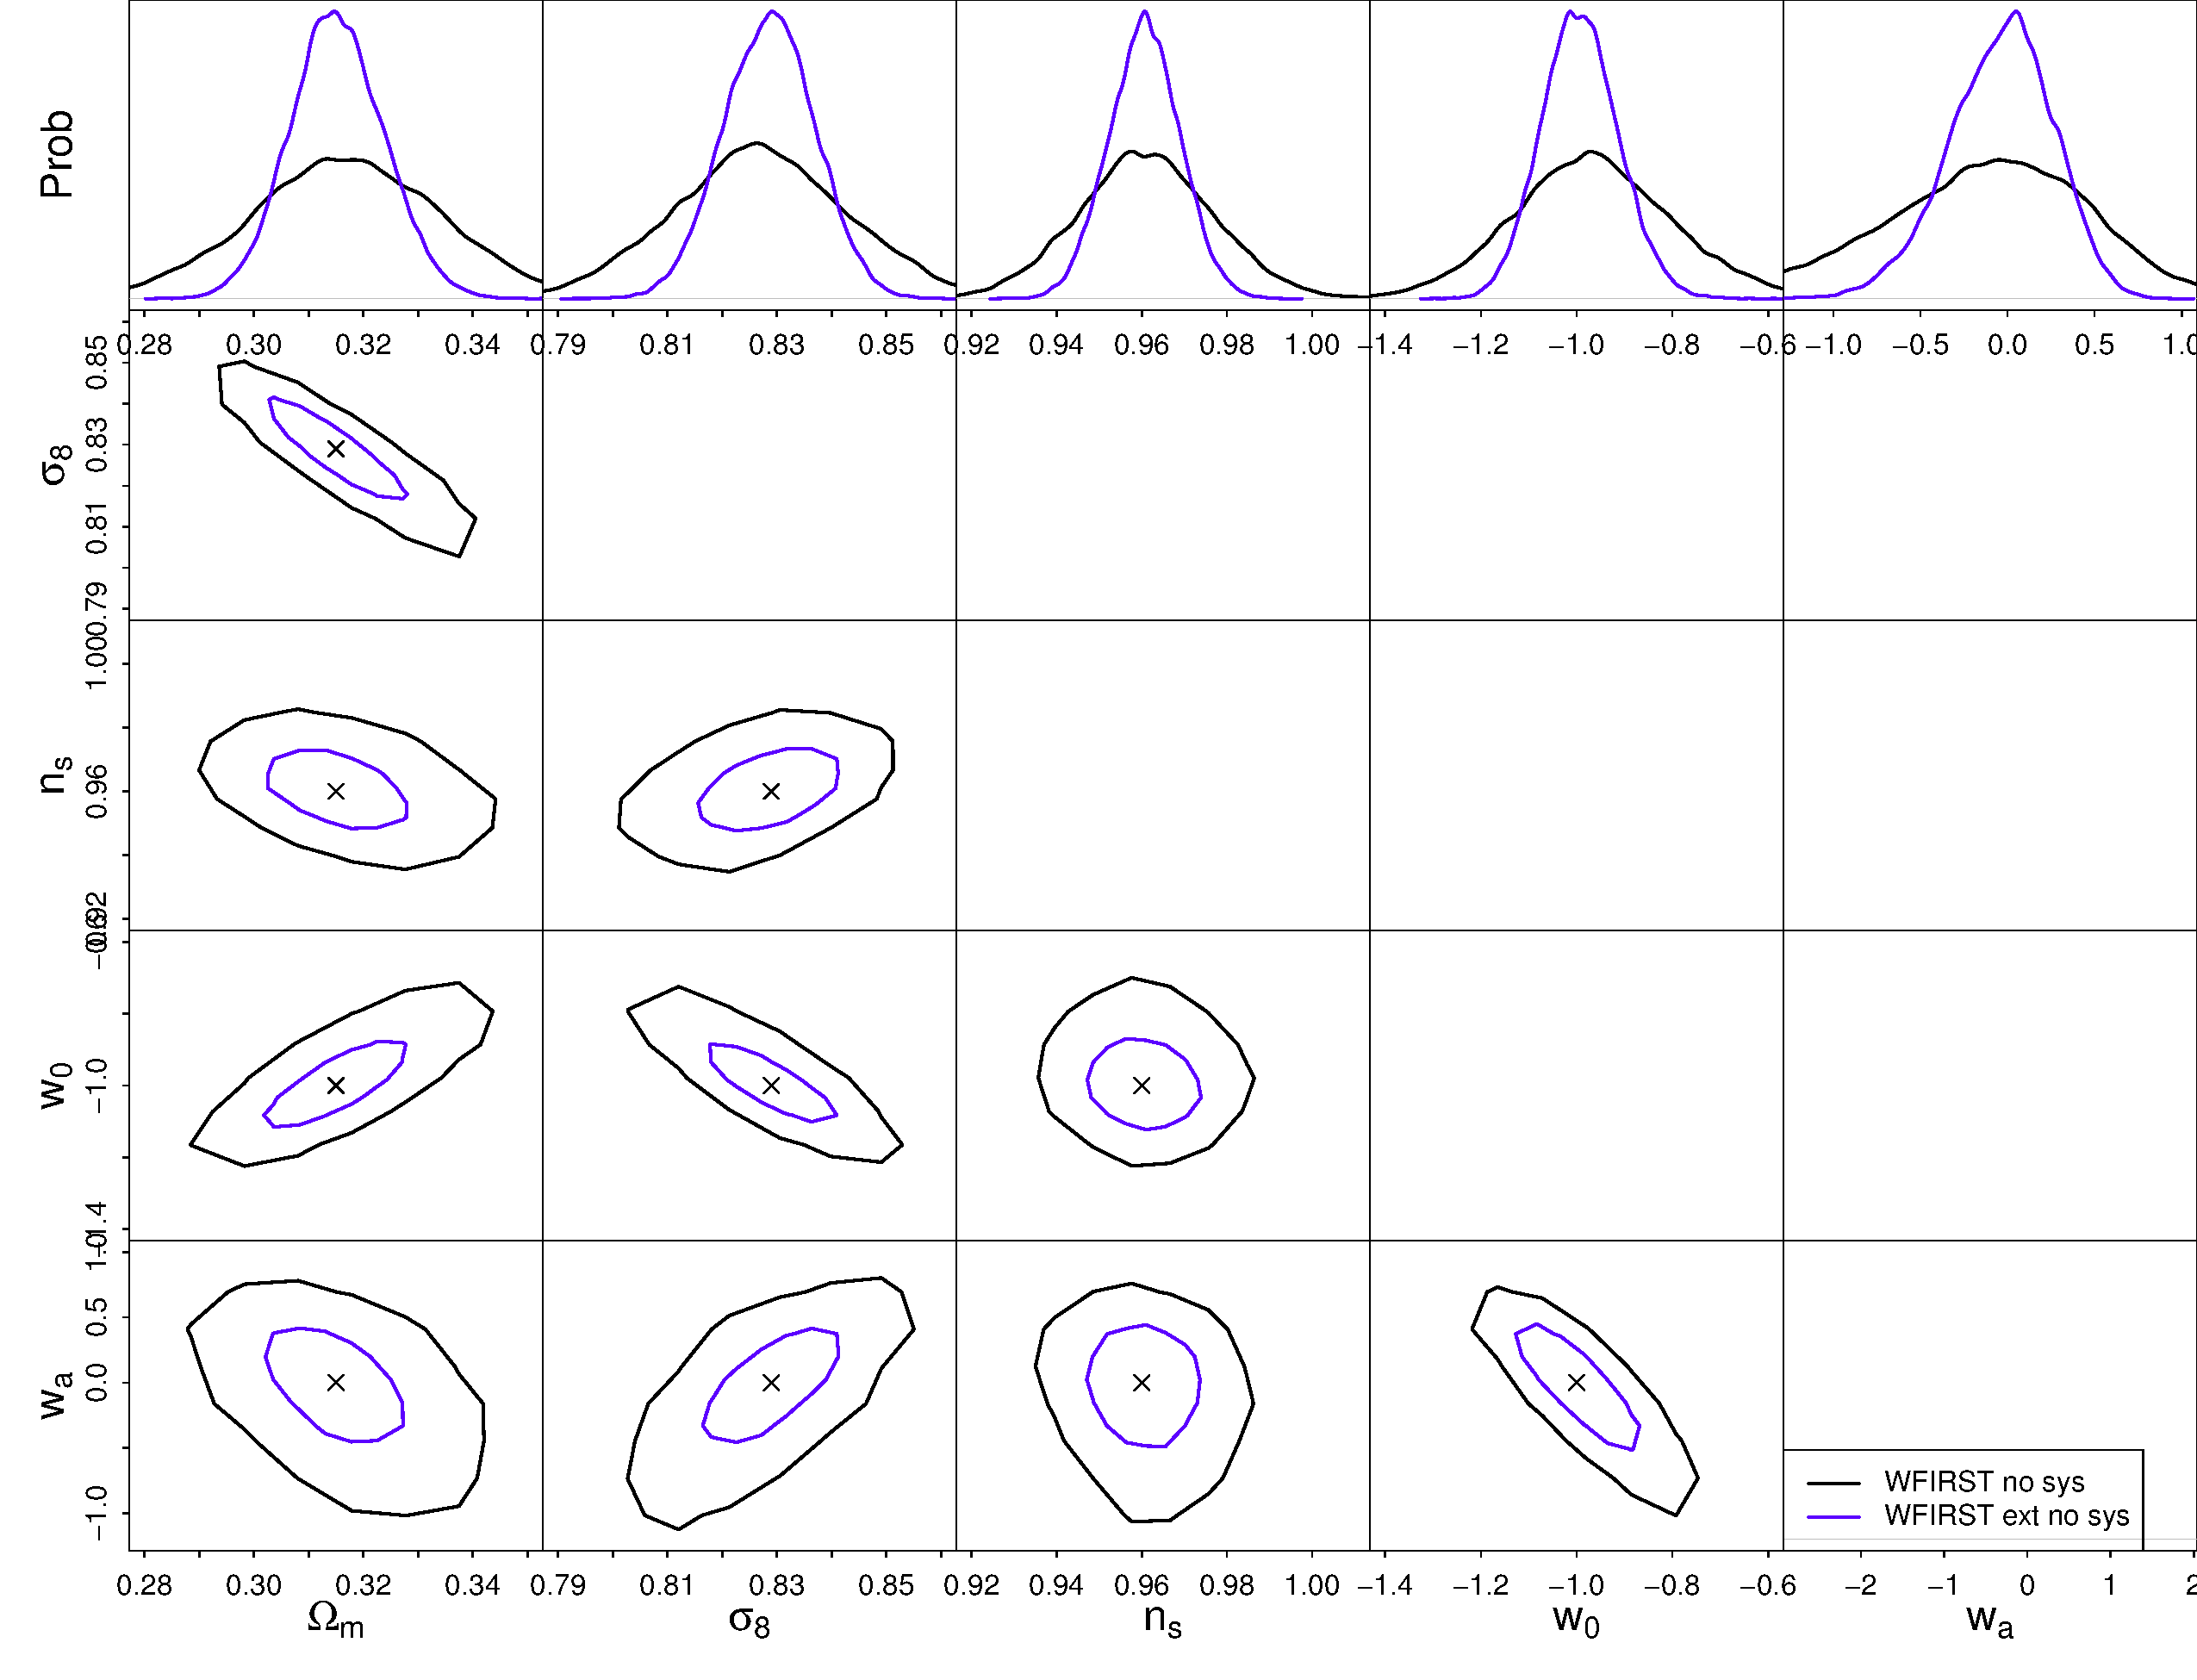
\includegraphics[width=14cm]{Plots/forecasts/WFIRST_no_sys.eps}
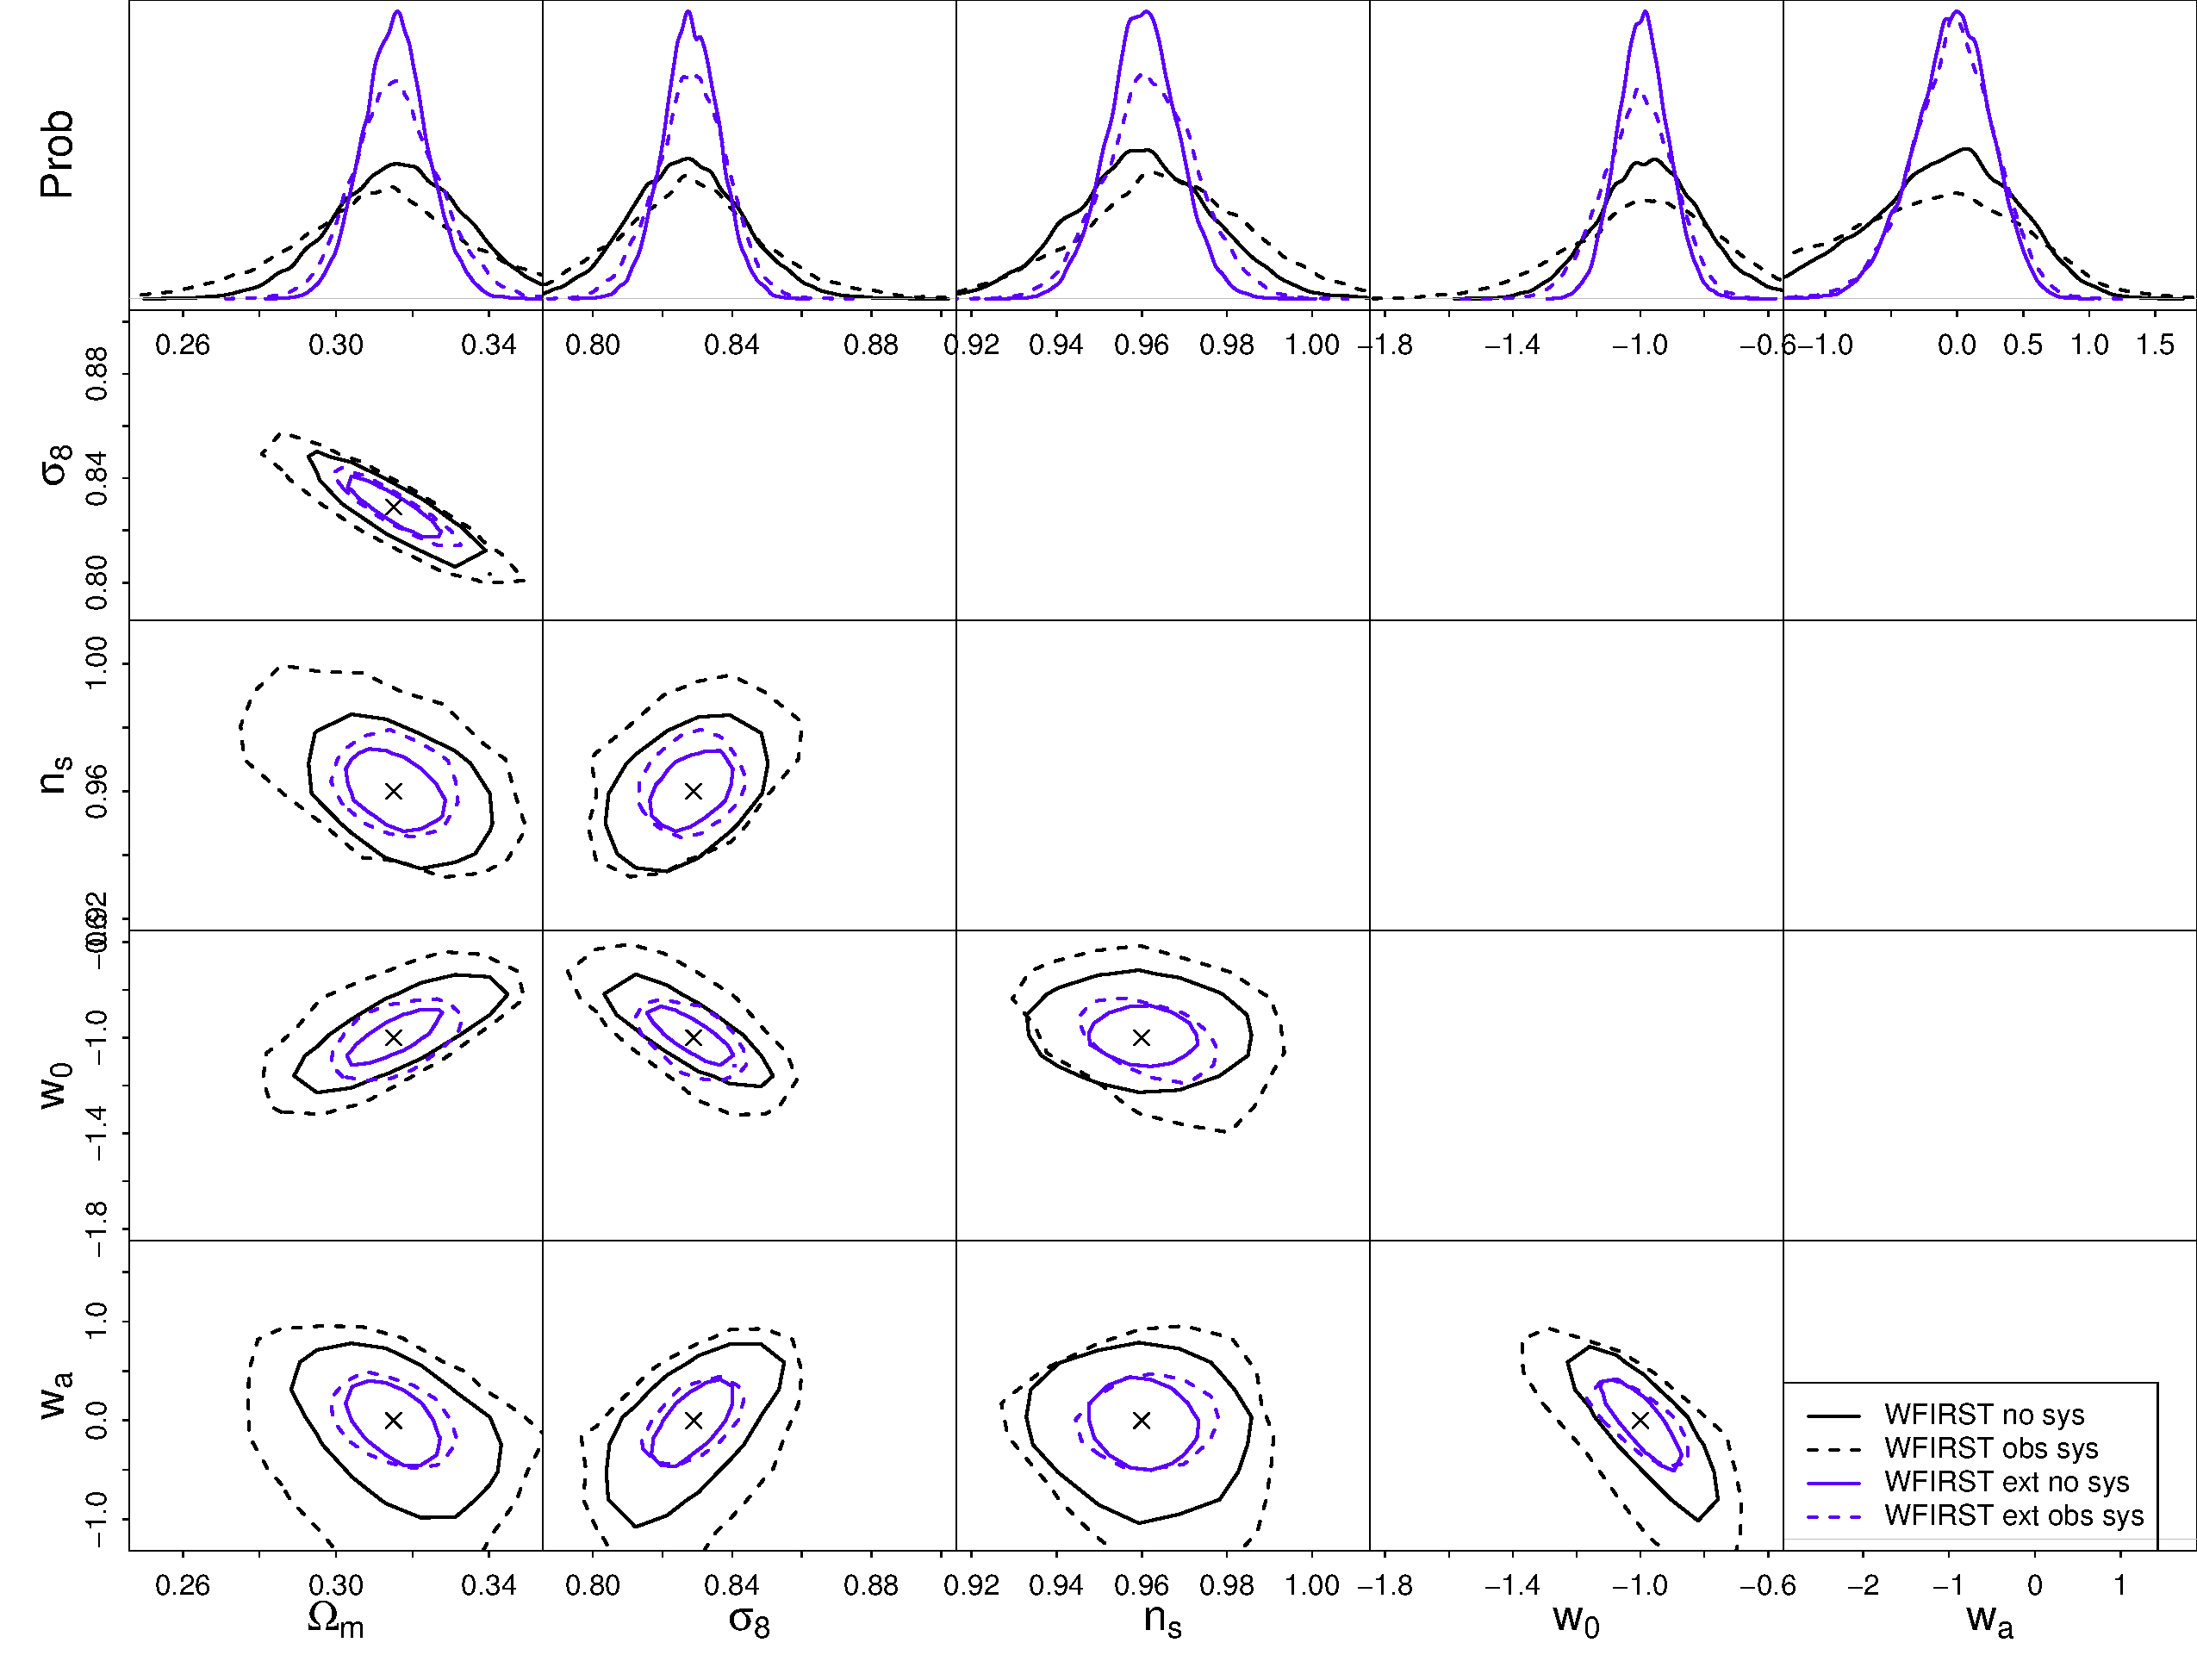
\includegraphics[width=14cm]{Plots/forecasts/WFIRST_obs_sys.eps}
\caption{\textit{Top:} WFIRST forecasts: statistical errors. Extended 10,000 $\mr{deg^2}$ mission in blue, regular 2,200 $\mr{deg^2}$ mission in black. \textit{Bottom:} Broadening of WFIRST error bars accounting for shear calibration and photo-z errors.}
         \label{fi:extended}
\end{figure}

\begin{figure}
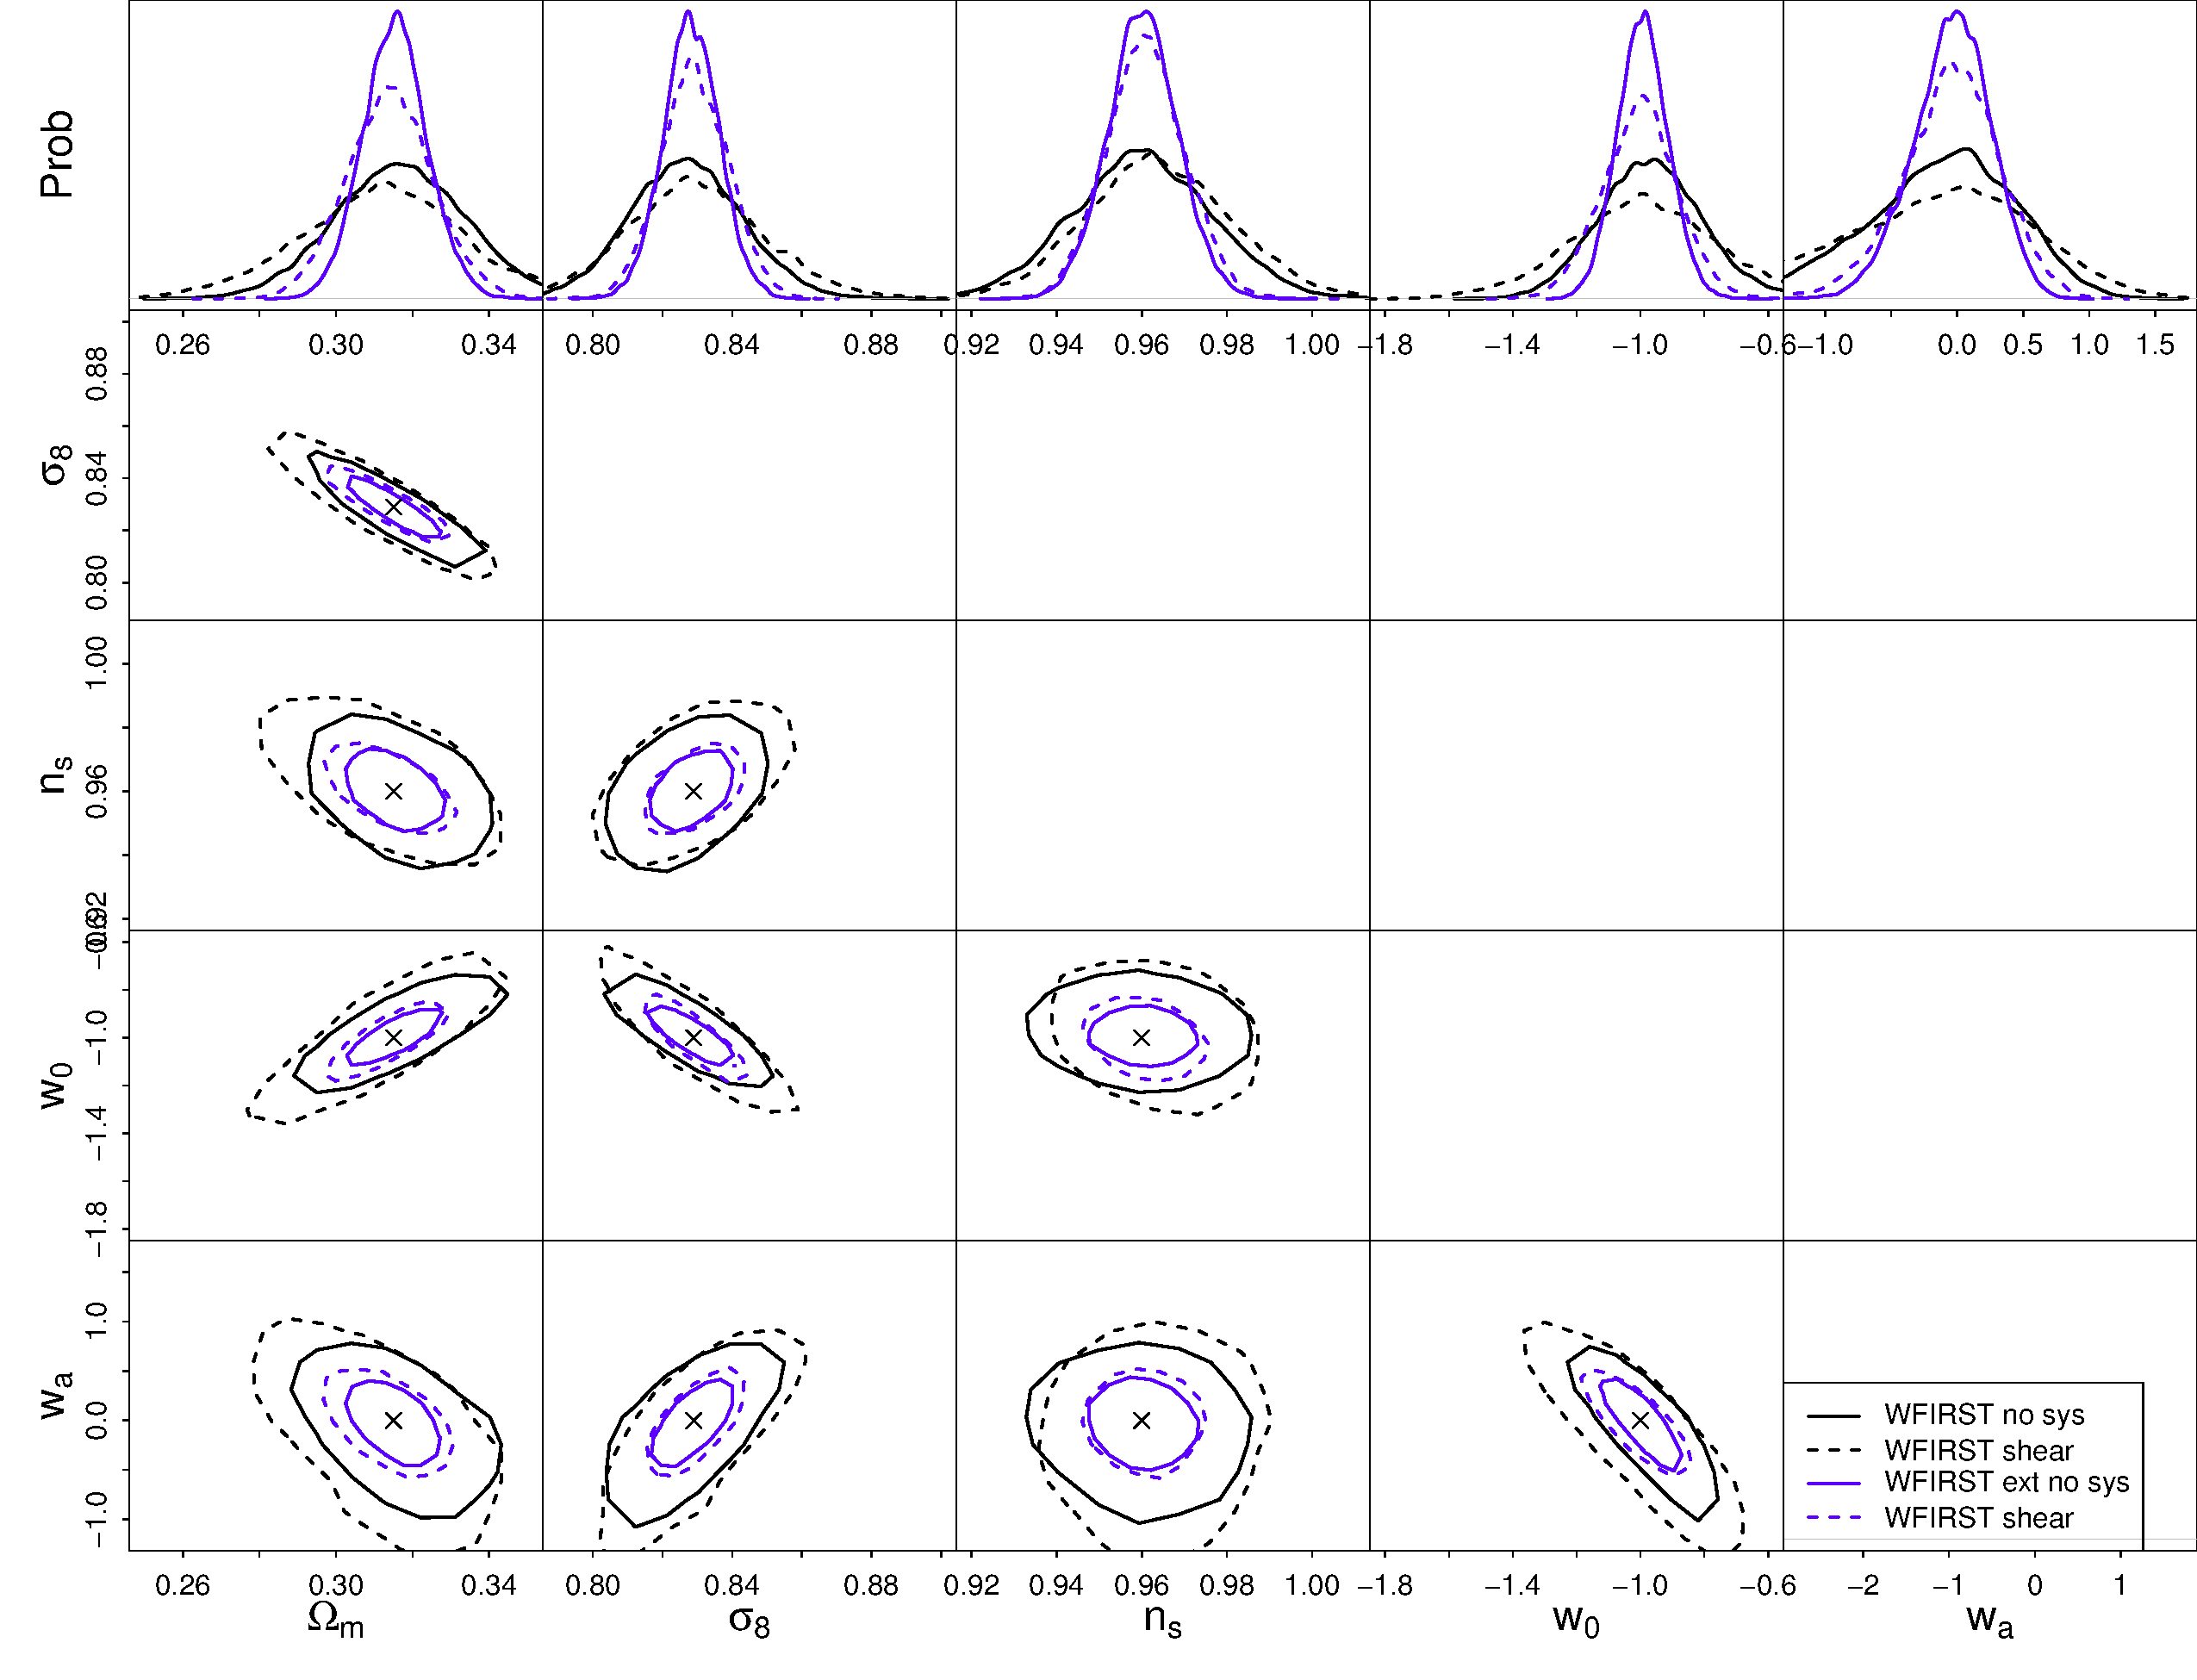
\includegraphics[width=14cm]{Plots/forecasts/WFIRST_shear.eps}
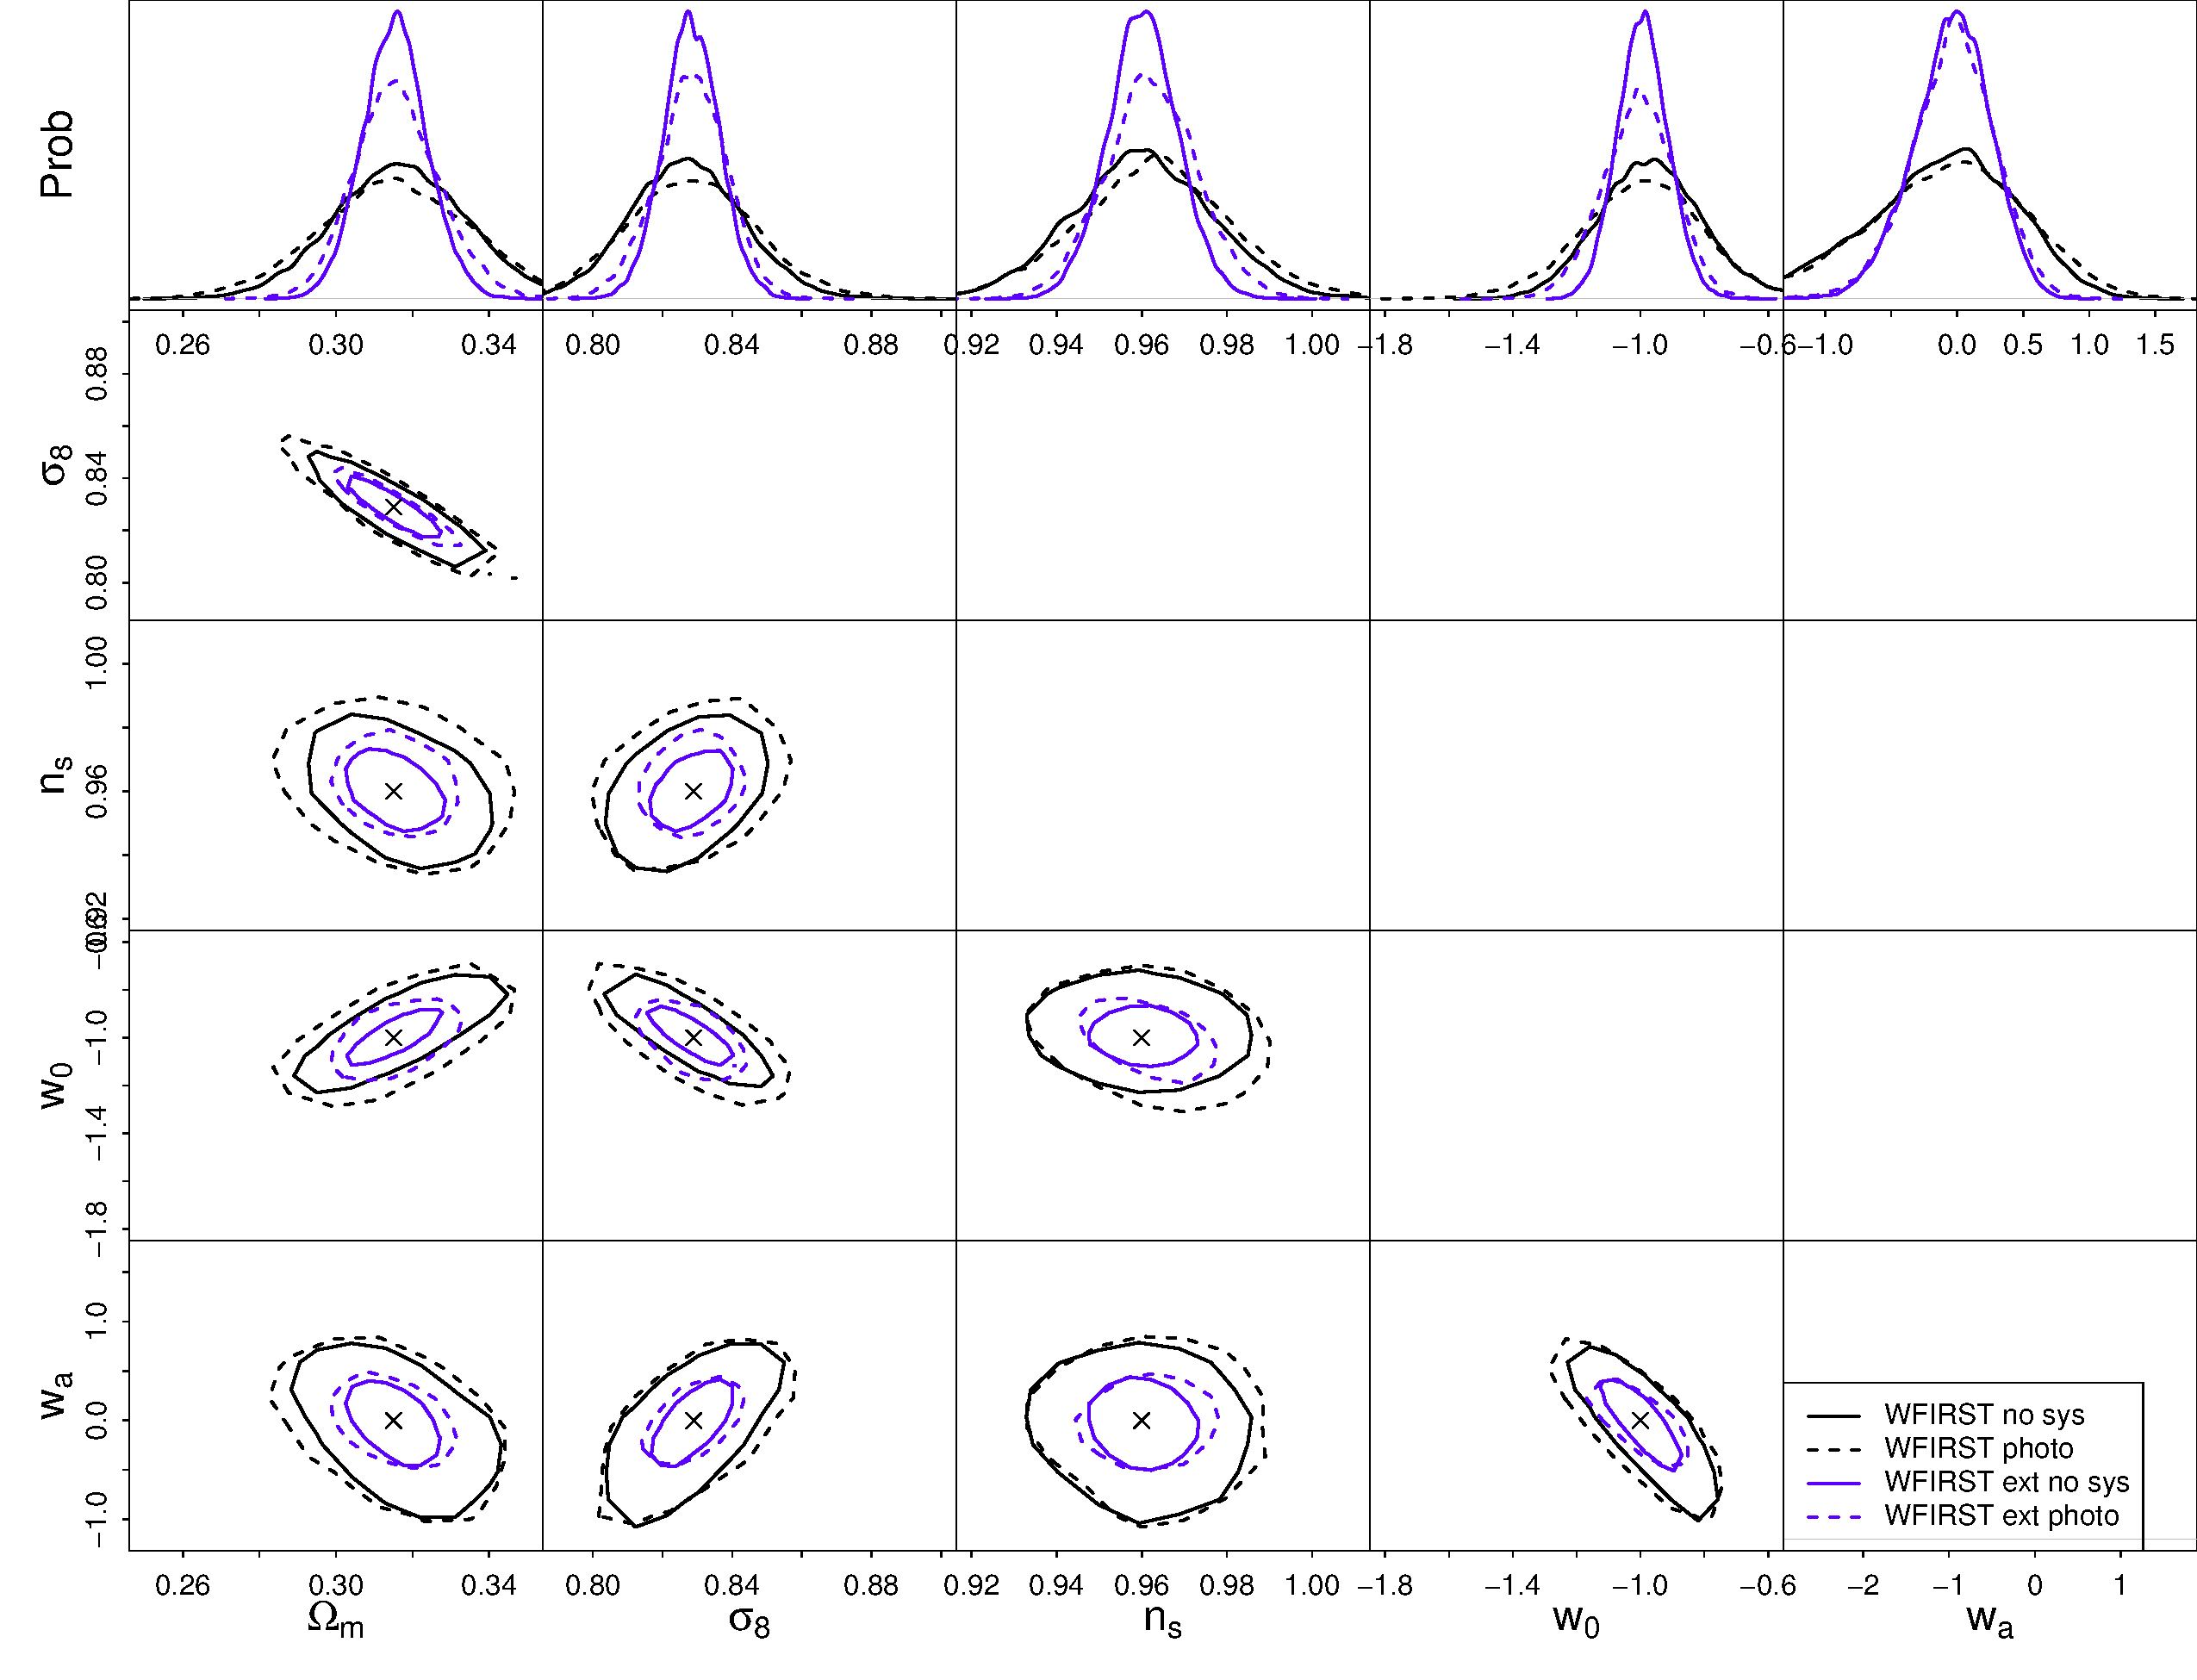
\includegraphics[width=14cm]{Plots/forecasts/WFIRST_photo.eps}
\caption{\textit{Top:} WFIRST statistical errors (solid) compared to errors when including uncertainties from multiplicative shear calibration errors (dashed).  Extended 10,000 $\mr{deg^2}$ mission in blue, regular 2,200 $\mr{deg^2}$ mission in black
\textit{Bottom:} WFIRST contours when accounting for photo-$z$ uncertainties; see text for details.}
         \label{fi:sys_obs}
\end{figure}

\begin{figure}
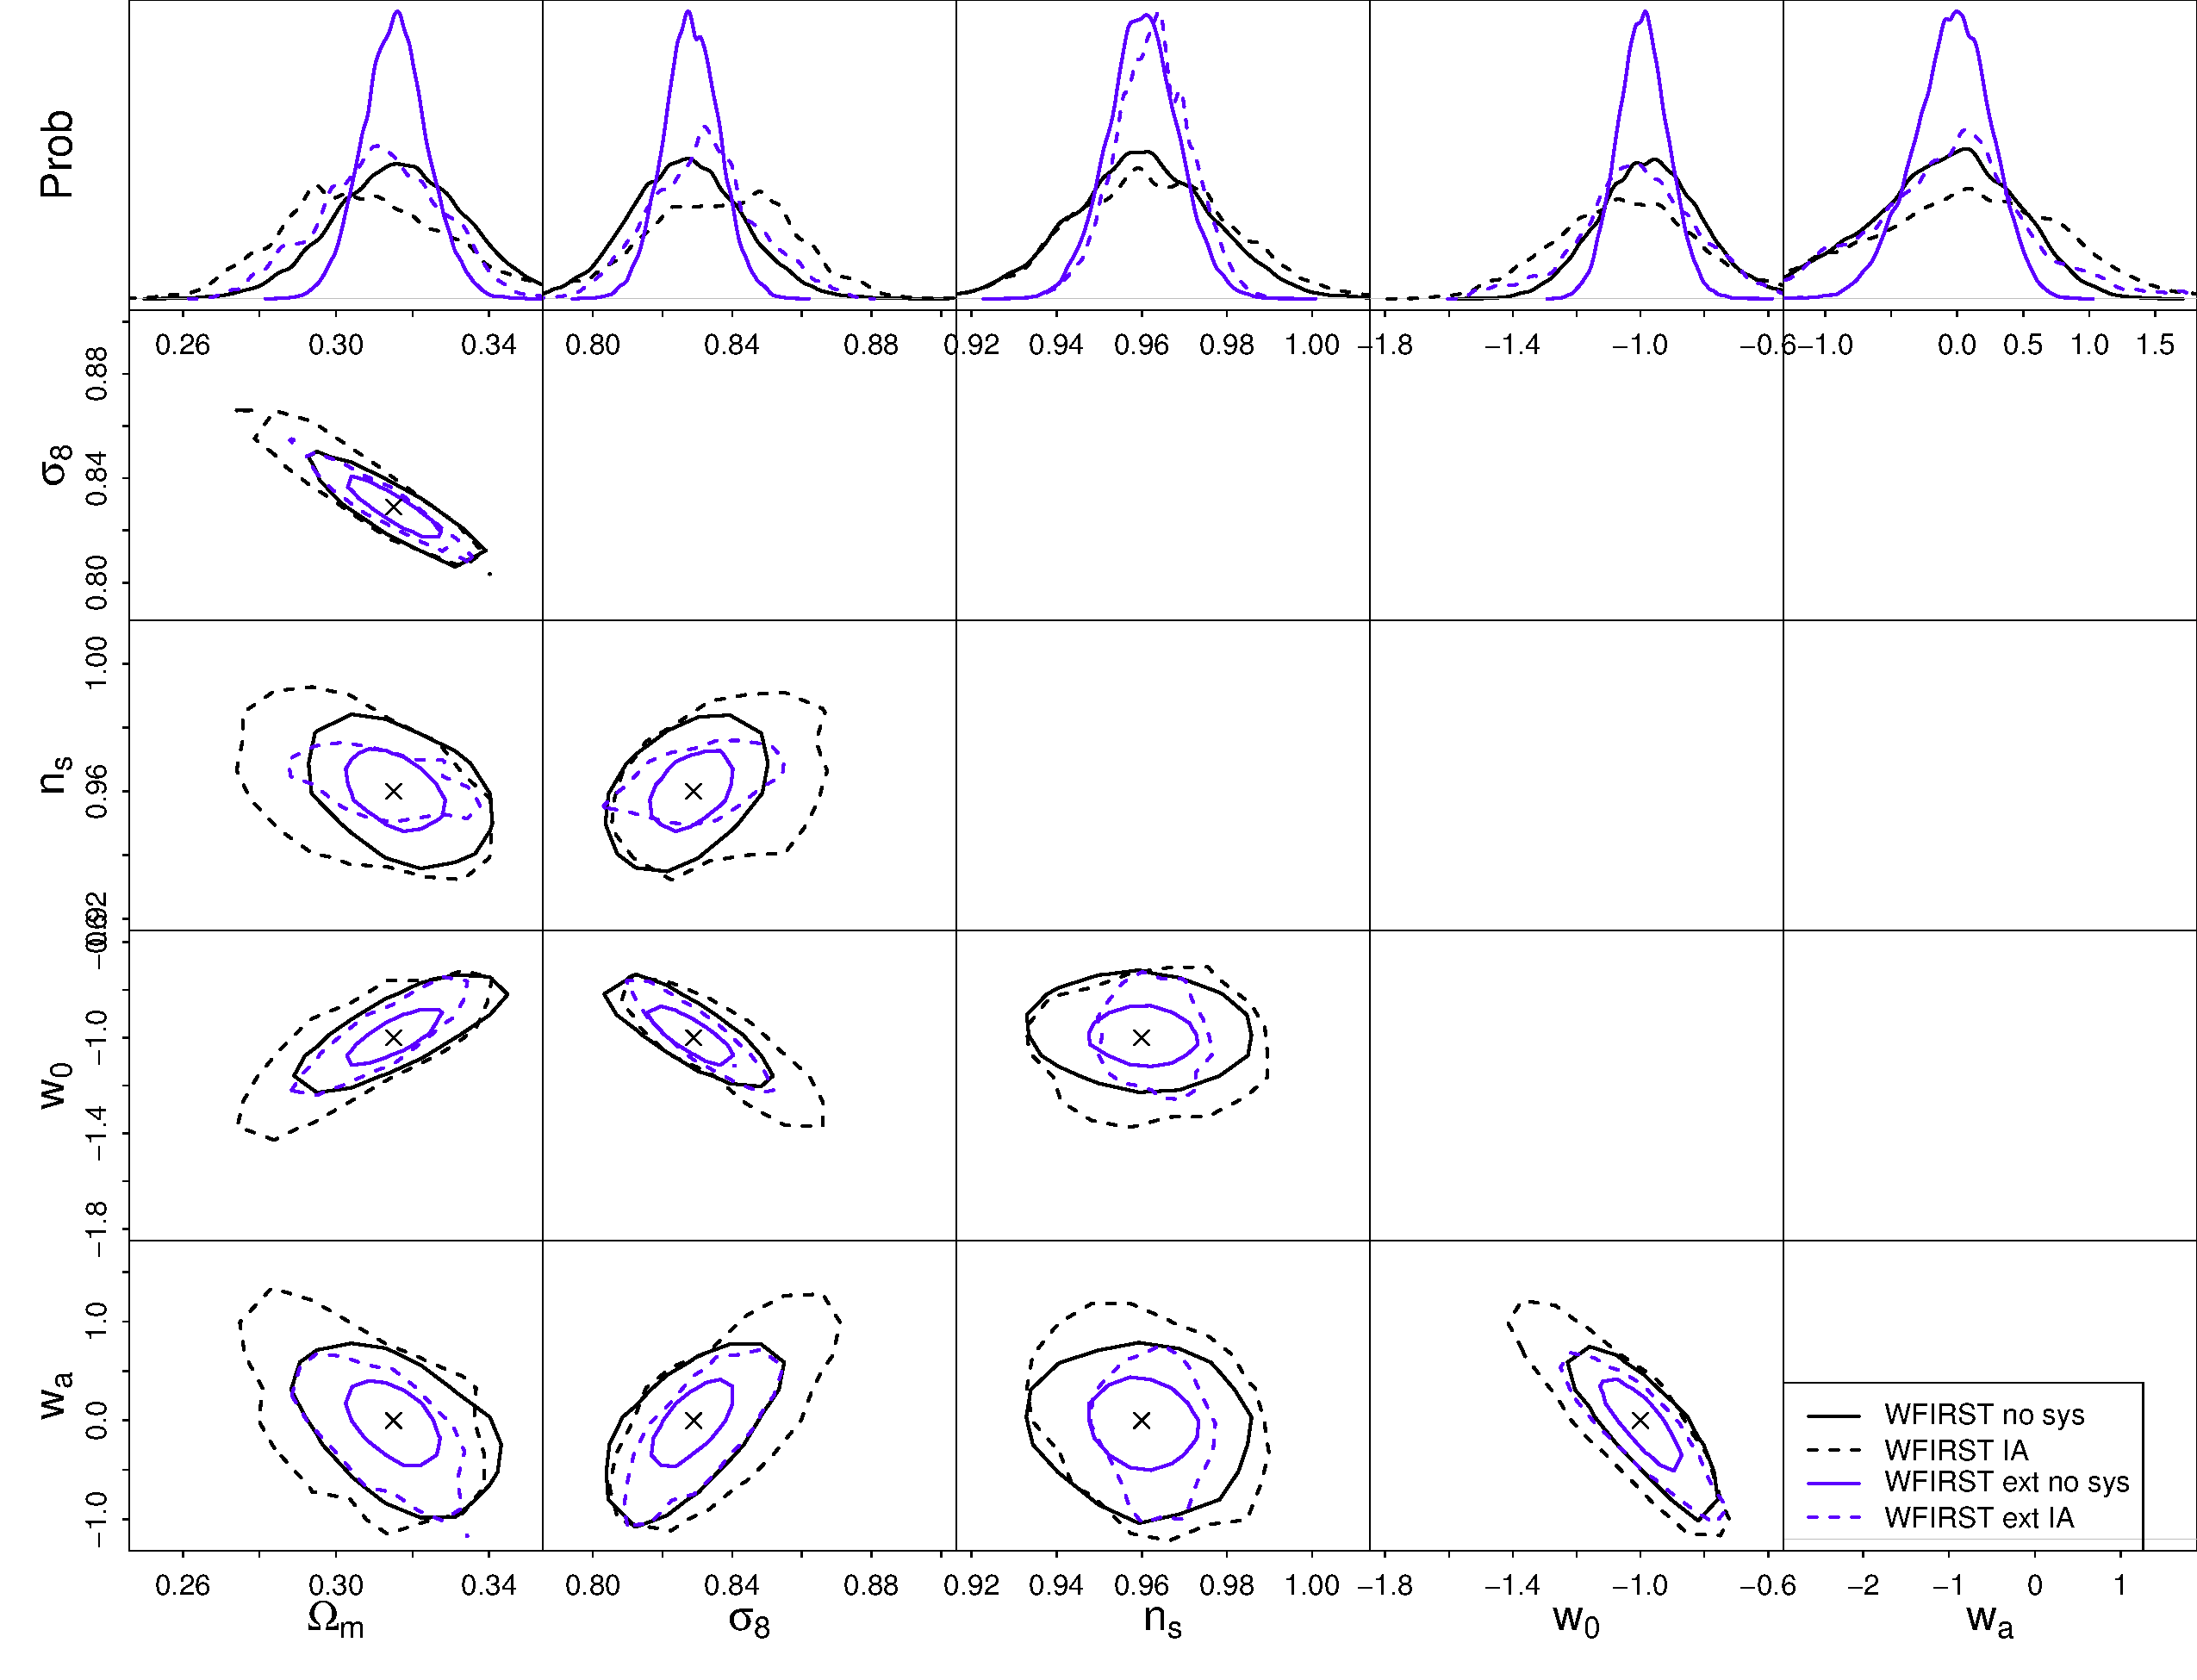
\includegraphics[width=14cm]{Plots/forecasts/WFIRST_ia.eps}
\caption{Increase of WFIRST (nominal and extended mission) error bars when marginalizing over intrinsic alignment nuisance parameters \citep[see][for comparison]{Krause2016}.} \label{fi:IA}
\end{figure}

\begin{figure}
\includegraphics[width=14cm]{Plots/forecasts/WFIRST_bary_impact.eps}
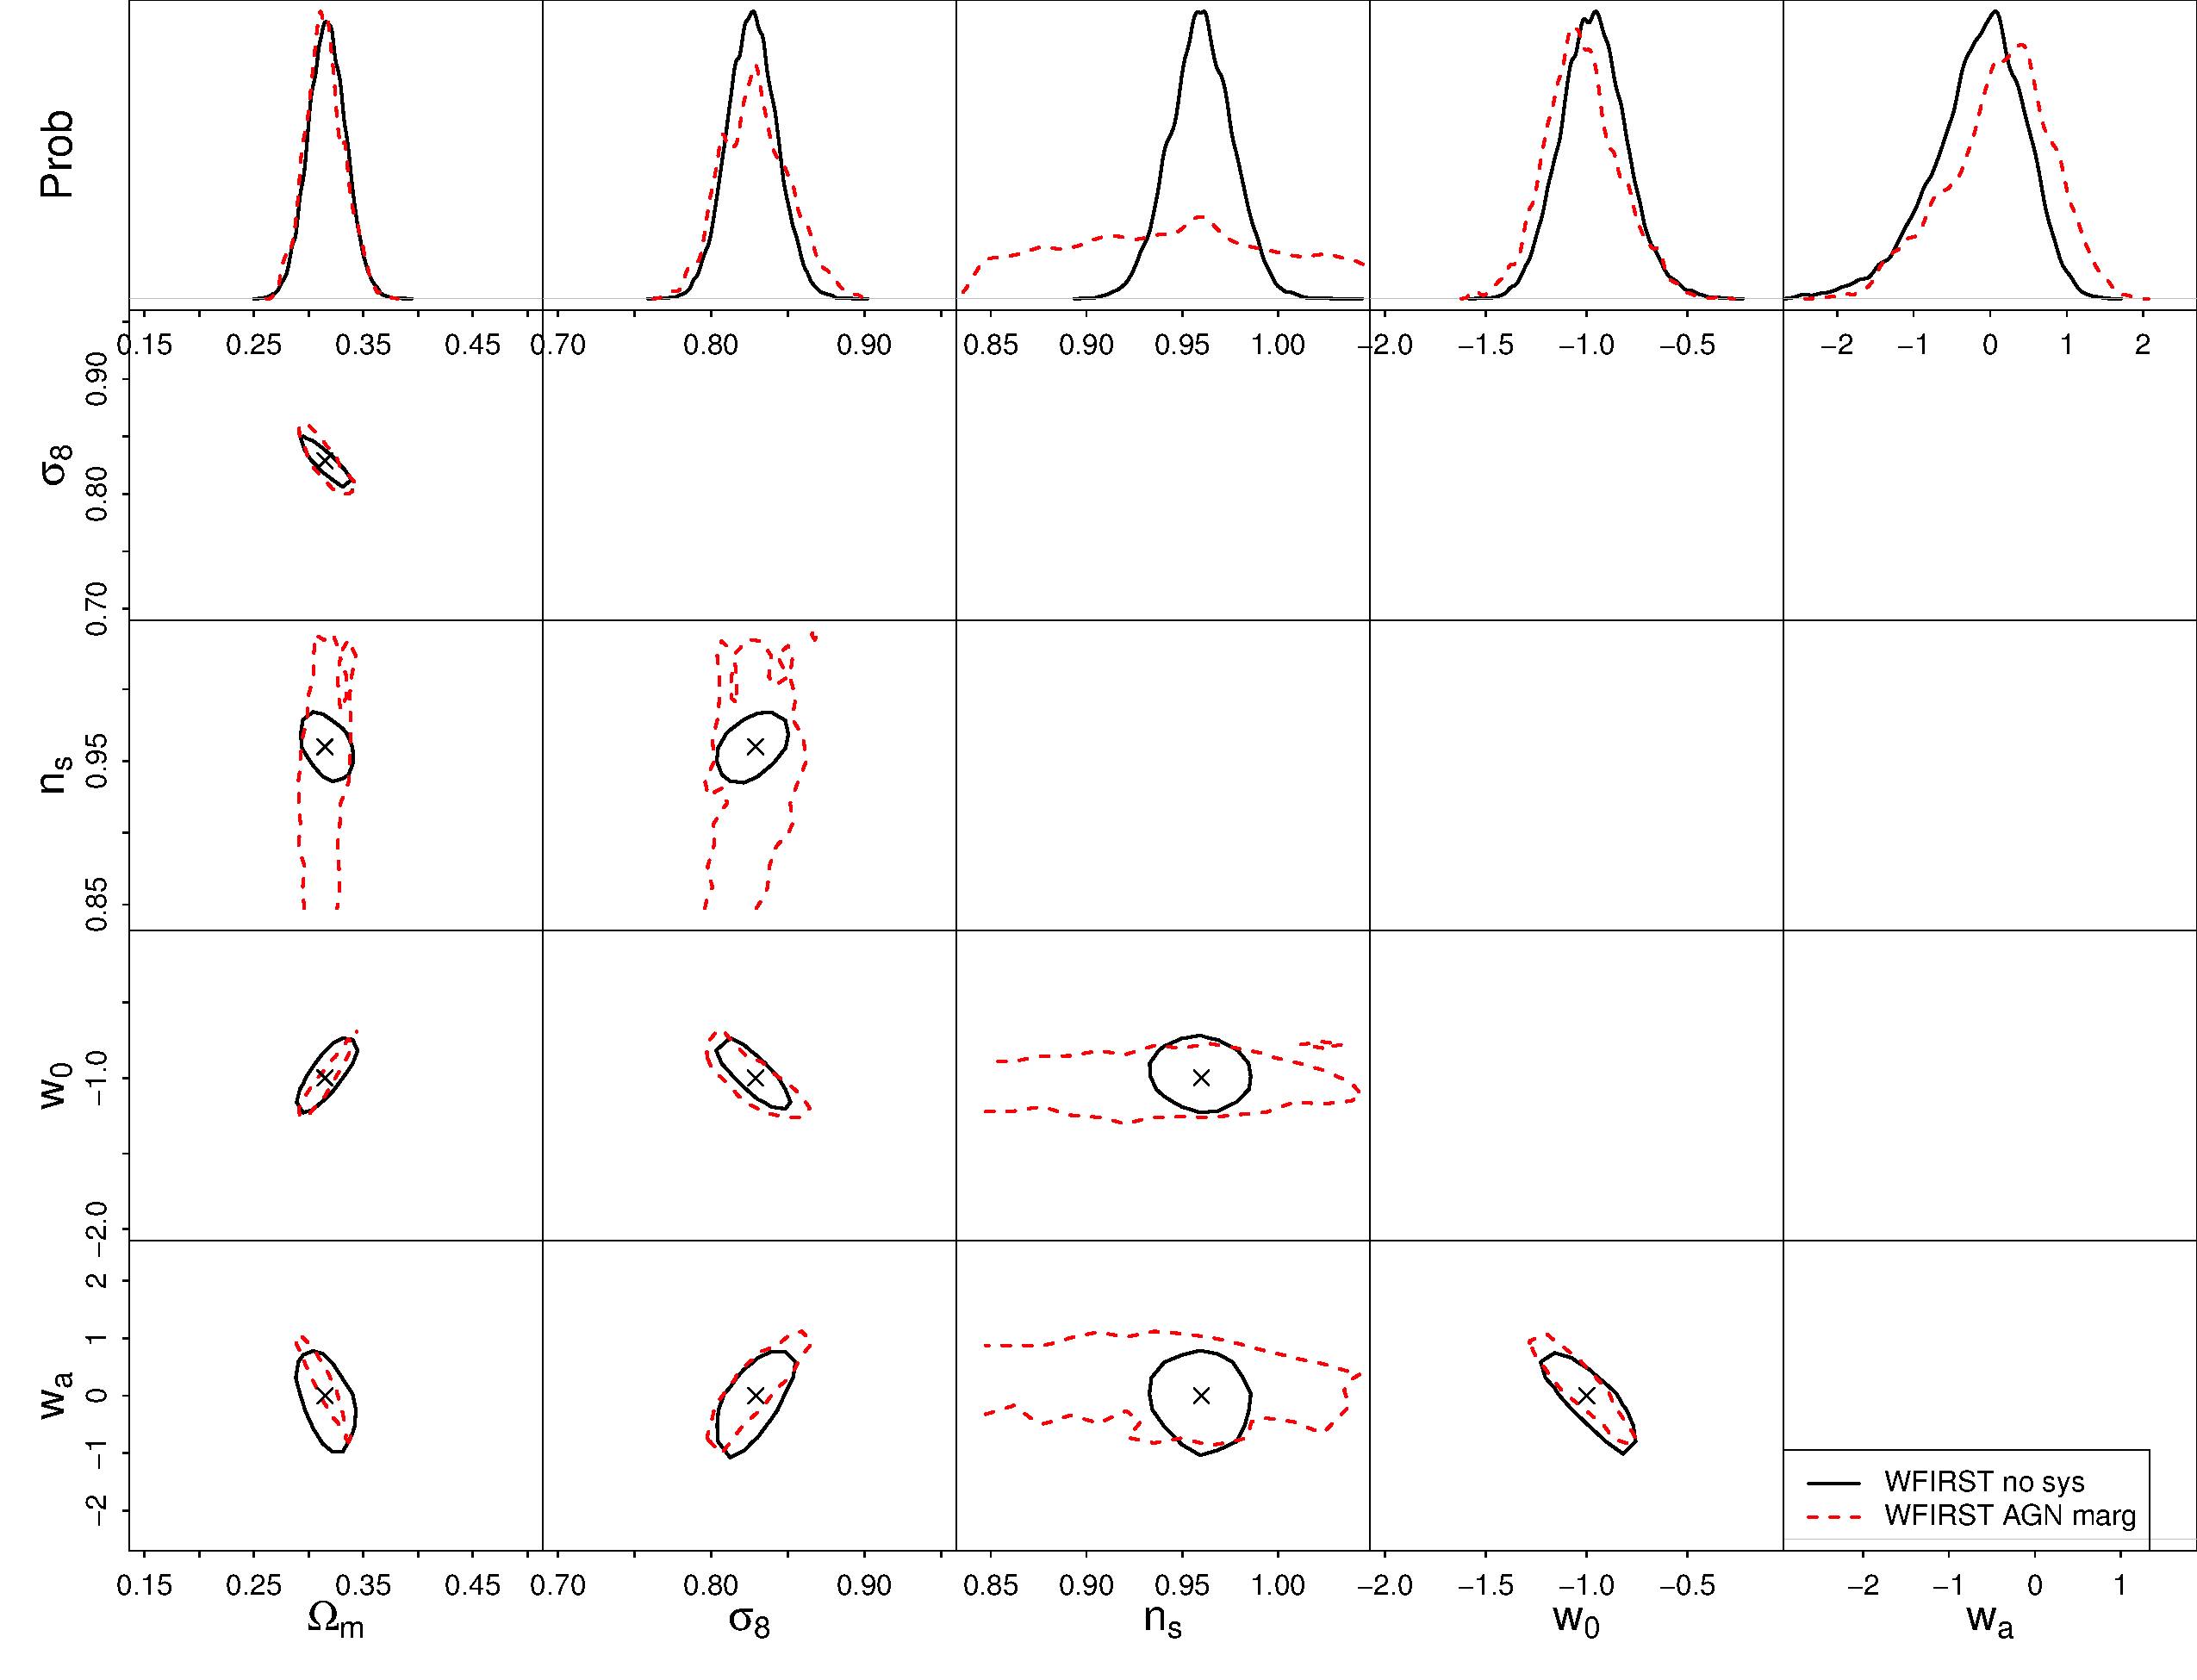
\includegraphics[width=14cm]{Plots/forecasts/WFIRST_bary_miti.eps}
\caption{Increase of WFIRST (nominal and extended mission) error bars when marginalizing over nuisance parameters modeling baryonic physics \citep[see][for details of the method]{Eifler2015}.}
         \label{fi:bary}
\end{figure}

\subsubsection{Modeling Weak lensing observables and covariances}
\label{sec:lensingbasics}

We begin this WFIRST HLIS section by forecasting the weak lensing science component only. We closely follow the weak lensing part of the forecasting machinery described in \cite{Krause2017}.

\paragraph{Shear Tomography Power Spectra} \CoLi obtains matter power spectra through calls to the Boltzmann \textsc{CLASS} code and it uses the \citet{tsn12} calibration of the \textsc{halofit} fitting function for the non-linear matter power spectrum \citep{smp03}. Time-dependent dark energy models ($w=w_0+(1-a)\,w_a$) are incorporated following the recipe of {\sc icosmo} \citep{rak11}, which in the non-linear regime interpolates Halofit between flat and open cosmological models \citep[also see][for more details]{shj10}.

Having obtained the density power spectra we calculate the shear power spectra as
\begin{equation}
\label{eq:pdeltatopkappa}
C ^{ij} (l) = \frac{9H_0^4 \om^2}{4c^4} \int_0^{\chi_\mr h}
\mr d \chi \, \frac{g^{i}(\chi) g^{j}(\chi)}{a^2(\chi)} \pd \left(\frac{l}{f_K(\chi)},\chi \right) \,,
\end{equation}
with $l$ being the 2D wave vector perpendicular to the line of sight, $\chi$ is the comoving coordinate, $\chi_\mr h$ is the comoving coordinate of the horizon, $a(\chi)$ is the scale factor, and $f_K(\chi)$ the comoving angular diameter distance (throughout set to $\chi$ since we assume a flat Universe). The lens efficiency $g^{i}$ is defined as an integral over the redshift distribution of source galaxies $n(\chi(z))$ in the $i^\mr{th}$ tomographic interval
\begin{equation}
\label{eq:redshift_distri}
g^{i}(\chi) = \int_\chi^{\chi_{\mr h}} \mr d \chi' n^{i} (\chi') \frac{f_K (\chi'-\chi)}{f_K (\chi')} \,.
\end{equation}
Since we chose five tomographic bins, the resulting data vector which enters the likelihood analysis consists of 15 tomographic shear power spectra, each with 12 logarithmically spaced bins ($l \in [100;5000]$), hence 180 data points overall. The limits of the tomographic $z$-bins are chosen such that each bin contains a similar number of galaxies.


\paragraph{Shear Covariances} Under the assumption that the 4pt-function of the shear field can be expressed in terms of 2pt-functions (so-called Gaussian shear field) the covariance of projected shear power spectra can be calculated as in \citep{huj04}
\be
\label{eq:covhujain}
\mr{Cov_G} \left( C^{ij} (l_1) C^{kl} (l_2) \right) = \langle \Delta C^{ij} (l_1) \, \Delta C^{kl} (l_2) \rangle  =  \frac{\delta_{l_1 l_2}}{ 2 f_\mr{sky} l_1 \Delta l_1}  \left[\bar C^{ik}(l_1) \bar C^{jl}(l_1) + \bar C^{il}(l_1) \bar C^{jk} (l_1) \right]\,,
\ee

with
\be
\label{details}
\bar C^{ij}(l_1)= C^{ij}(l_1)+ \delta_{ij} \frac{\sigma_\eps^2}{n^{i}} \,,
\ee
where the superscripts indicate the redshift bin; $n^{i}$ is the density of source galaxies in the $i$-th redshift bin; and $\sigma_\eps$ is the RMS of the shape noise.

Since non-linear structure growth at late time induces significant non-Gaussianities in the shear field, using the covariance of Eq.~(\ref{eq:covhujain}) in a likelihood analysis results in an underestimate of the errors on cosmological parameters. Therefore, the covariance must be amended by an additional term, i.e. $\mr{Cov}=\mr{Cov_G}+\mr{Cov_{NG}}$.  The non-Gaussian covariance is calculated from the convergence trispectrum $T_{\kappa}$ \citep{CH01,taj09}, and we include a sample variance term $T_{\kappa,\rm{HSV}}$ that describes scatter in power spectrum measurements due to large scale density modes \citep{tb07, sht09},
\be
 \mr{Cov_{NG}}(C^{ij}(l_1),C^{kl}(l_2)) =  \int_{|\mathbf l|\in l_1}\frac{d^2\mathbf l}{A(l_1)}\int_{|\mathbf l'|\in l_2}\frac{d^2\mathbf l'}{A(l_2)} \left[\frac{1}{\Omega_{\mr s}}T_{\kappa,0}^{ijkl}(\mathbf l,-\mathbf l,\mathbf l',-\mathbf l') + T_{\kappa,\rm{HSV}}^{ijkl}(\mathbf l,-\mathbf l,\mathbf l',-\mathbf l') \right] \,,
\ee
with $A(l_i) = \int_{|\mathbf l|\in l_i}d^2\mathbf l \approx 2 \pi l_i\Delta l_i$ the integration area associated with a power spectrum bin centered at $l_i$ and width $\Delta l_i$.

The convergence trispectrum $T_{\kappa,0}^{ijkl}$ (in the absence of finite volume effects) is defined as
\be
\label{eq:tri2}
T_{\kappa,0}^{ijkl} (\mathbf l_1,\mathbf l_2,\mathbf l_3,\mathbf l_4) = \left( \frac{3}{2} \frac{H_0^2}{c^2} \om \right)^{4} \int_0^{\chi_h} \d \chi \, \left( \frac{\chi}{a(\chi)}\right)^4  g^i g^j g^k g^l \times \chi^{-6} \, T_{\delta,0}  \left( \frac{\mathbf l_1}{\chi}, \frac{\mathbf l_2}{\chi}, \frac{\mathbf l_3}{\chi}, \frac{\mathbf l_4}{\chi}, z(\chi) \right) \,,
\ee
with $T_{\delta,0}$ the matter trispectrum (again, not including finite volume effects), and where we abbreviated $g^i=g^i(\chi)$.

We model the matter trispectrum using the halo model \citep{Seljak00, CS02}, which assumes that all matter is bound in virialized structures that are modeled as biased tracers of the density field. Within this model the statistics of the density field can be described by the dark matter distribution within halos on small scales, and is dominated by the clustering properties of halos and their abundance on large scales. In this model, the trispectrum splits into five terms describing the 4-point correlation within one halo (the \emph{one-halo} term $T^{\mr{1h}}$), between 2 to 4 halos (\emph{two-, three-, four-halo} term), and a so-called halo sample variance term $T_{\mr{HSV}}$, caused by fluctuations in the number of massive halos within the survey area,
\be
\label{eq:t}
T = T_0 + T_{\mr{HSV}} = \left[T_{\mr{1h}}+T_{\mr{2h}}+T_{\mr{3h}}+T_{\mr{4h}}\right]+T_{\mr{HSV}}\;.
\ee
The \emph{two-halo} term is split into two parts, representing correlations between two or three points in the first halo and two or one point in the second halo. As halos are the building blocks of the density field in the halo model approach, we need to choose models for their internal structure, abundance, and clustering, in order to build a model for the trispectrum.


Our implementation of the one-, two- and four-halo term contributions to the matter trispectrum follows \citet{CH01}, and we neglect the three-halo term as it is subdominant compared to the other terms at the scales of interest for this analysis. Specifically, we assume NFW halo profiles \citep{NFW} with the \citet{Bhattacharya11} fitting formula for the halo mass--concentration relation $c(M,z)$, and the \citet{Tinker2008} fitting functions for the halo mass function $\frac{ dn}{dM}$ and linear halo bias $b(M)$ (all evaluated at $\Delta = 200$), neglecting terms involving higher order halo biasing.


Within the halo model framework, the halo sample variance term is described by the change of the number of massive halos within the survey area due to survey-scale density modes. Following \citet{sht09}, it is calculated as

\begin{eqnarray}
T_{\kappa,\rm{HSV}}^{ijkl}(\mathbf l_1,-\mathbf l_1,\mathbf l_2,-\mathbf l_2)= \left(\frac{3}{2}\frac{H_0^2}{c^2}\Omega_{\mr m}\right)^4 &\times&  \int_0^{\chi_\mr h}d\chi \left(\frac{d^2 V}{d\chi d\Omega}\right)^2 \left(\frac{\chi}{a(\chi)}\right)^4 g^i g^j g^k g^l \nn \\
&\times&  \int d M \frac{d n}{d M} b(M)\left(\frac{M}{\bar{\rho}}\right)^2 |\tilde{u}(l_1/\chi, c(M,z(\chi))|^2 \nn \\
 &\times& \int d M' \frac{d n}{d M'} b(M')\left(\frac{M'}{\bar{\rho}}\right)^2 |\tilde{u}(l_2/\chi, c(M',z(\chi))|^2 \nn \\
 &\times&  \int_0^\infty \frac{k dk}{2\pi}P_\delta^{\mr{lin}}(k,z(\chi))|\tilde W(k\chi \Theta_{\mr s})|^2 \,.
\end{eqnarray}


\paragraph{Cosmological Parameter Studies} Our ability to model shear power spectra and non-Gaussian covariances means that we can forcast cosmological constraints for different survey scenarios. For all forecasts, we sample the joint parameter space of cosmological $\pco$ and nuisance parameters $\pnu$ and parameterize the joint likelihood as a multivariate Gaussian
\be
\label{eq:like}
\like (\D| \pco, \pnu) = N \, \times \, \exp \biggl( -\frac{1}{2} \underbrace{\left[ (\D -\M)^t \, \matC^{-1} \, (\D-\M) \right]}_{\chi^2(\pco, \pnu)}  \biggr) \,.
\ee
The model vector $\M$ is a function of cosmology and nuisance parameters, i.e. $\M=\M(\pco, \pnu)$ and the normalization constant $N=(2 \pi)^{-\frac{n}{2}} |C|^{-\frac{1}{2}}$ can be ignored under the assumption that the covariance is constant in parameter space. The assumption of a constant, known covariance matrix $\matC$ is an approximation to the correct approach of a cosmology dependent or estimated covariance \citep[see][for further details]{esh09, seh16}.
Given the likelihood function we can compute the posterior probability in parameter space from Bayes' theorem
\be
\label{eq:bayes}
\prob(\pco, \pnu|\D) \propto \probr (\pco, \pnu) \,\like (\D| \pco, \pnu),
\ee
where $\probr (\pco, \pnu)$ denotes the prior probability.

Equation \ref{eq:bayes} allows us to simulate realistic likelihood analyses for various survey scenarios. In particular we consider the following scenarios:
\begin{itemize}
\item Science gain when extending the survey to 10,000 deg$^2$, instead of 2,200 deg$^2$ (see Fig \ref{fi:extended} top)
\item Impact of combined uncertainties in shape measurements and photo-z measurements (see Fig \ref{fi:extended} bottom)
\item Impact of uncertainties in shape measurements only (see Fig \ref{fi:sys_obs} top)
\item Impact of uncertainties in photo-z estimation only (see Fig \ref{fi:sys_obs} bottom)
\item Impact of uncertainties in baryonic physics modeling (see Fig \ref{fi:bary} bottom)
\item Impact of uncertainties in intrinsic alignment modeling (see Fig \ref{fi:IA} bottom)
\end{itemize}

Shear calibration uncertainties are modeled as a Gaussian with $\sigma=0.005$ in each of the 10 tomographic bins, which altogether leads to 11 nuisance parameters. Redshift errors are modeled as Gaussian errors with a bias around mean zero and $\sigma=0.05$. In each tomographic bin these parameters (bias and $sigma$) again have Gaussian priors, i.e. $\Delta \mr{bias}=0.005$ and $\Delta \sigma=0.006$.

For intrinsic alignment we assume the non-linear alignment model, closely following the parameterization and implementation of \cite{Krause2016}, i.e. we marginalize over 11 nuisance parameters for amplitude, redshift dependence, and luminosity function uncertainties.

For the impact of baryonic physics modeling, we follow the work of \cite{Eifler2015}, where the authors
examined the impact of different baryonic scenarios and quantify the bias in
cosmological constraints for LSST and DES when the impact of baryons are neglected. We repeat this analysis for WFIRST (Figure~\ref{fi:bary}, upper) and
also account for the uncertainties due to baryonic scenarios in a subsequent
analysis (Figure~\ref{fi:bary}, lower). There, we project out modes that are
sensitive to baryonic physics in our analysis, which comes at the cost of
constraining power, in particular the spectral index $n_s$. We note, however, that
$n_s$ is strongly constrained by CMB measurements and that a corresponding prior
will recover the lost information.


\subsection{Expanding the Science Case - Multi-Probe Forecasts}
\label{sec:multi-probe}

\begin{summaryii}
Using our updates to the \CoLi package described in the previous sections, we have now implemented a full multi-probe analysis, an extremely promising area of active research. We are able to combine \emph{all} cosmological probes enabled by WFIRST HLS. This is one of the major goal of our unified HLS SIT. The likelihood analyses presented here are the start of a demanding study to optimally combine WFIRST internal observables and also to study synergies between WFIRST and other, external data sets, in particular LSST\@. Our tools will enable us to do so in the coming years. We also study new cosmological signals these multi-probe analysis will allow us to measure, such as the effect of primordial non-Gaussianity on galaxy shapes and synergies with CMB lensing.
\end{summaryii}


\begin{figure}
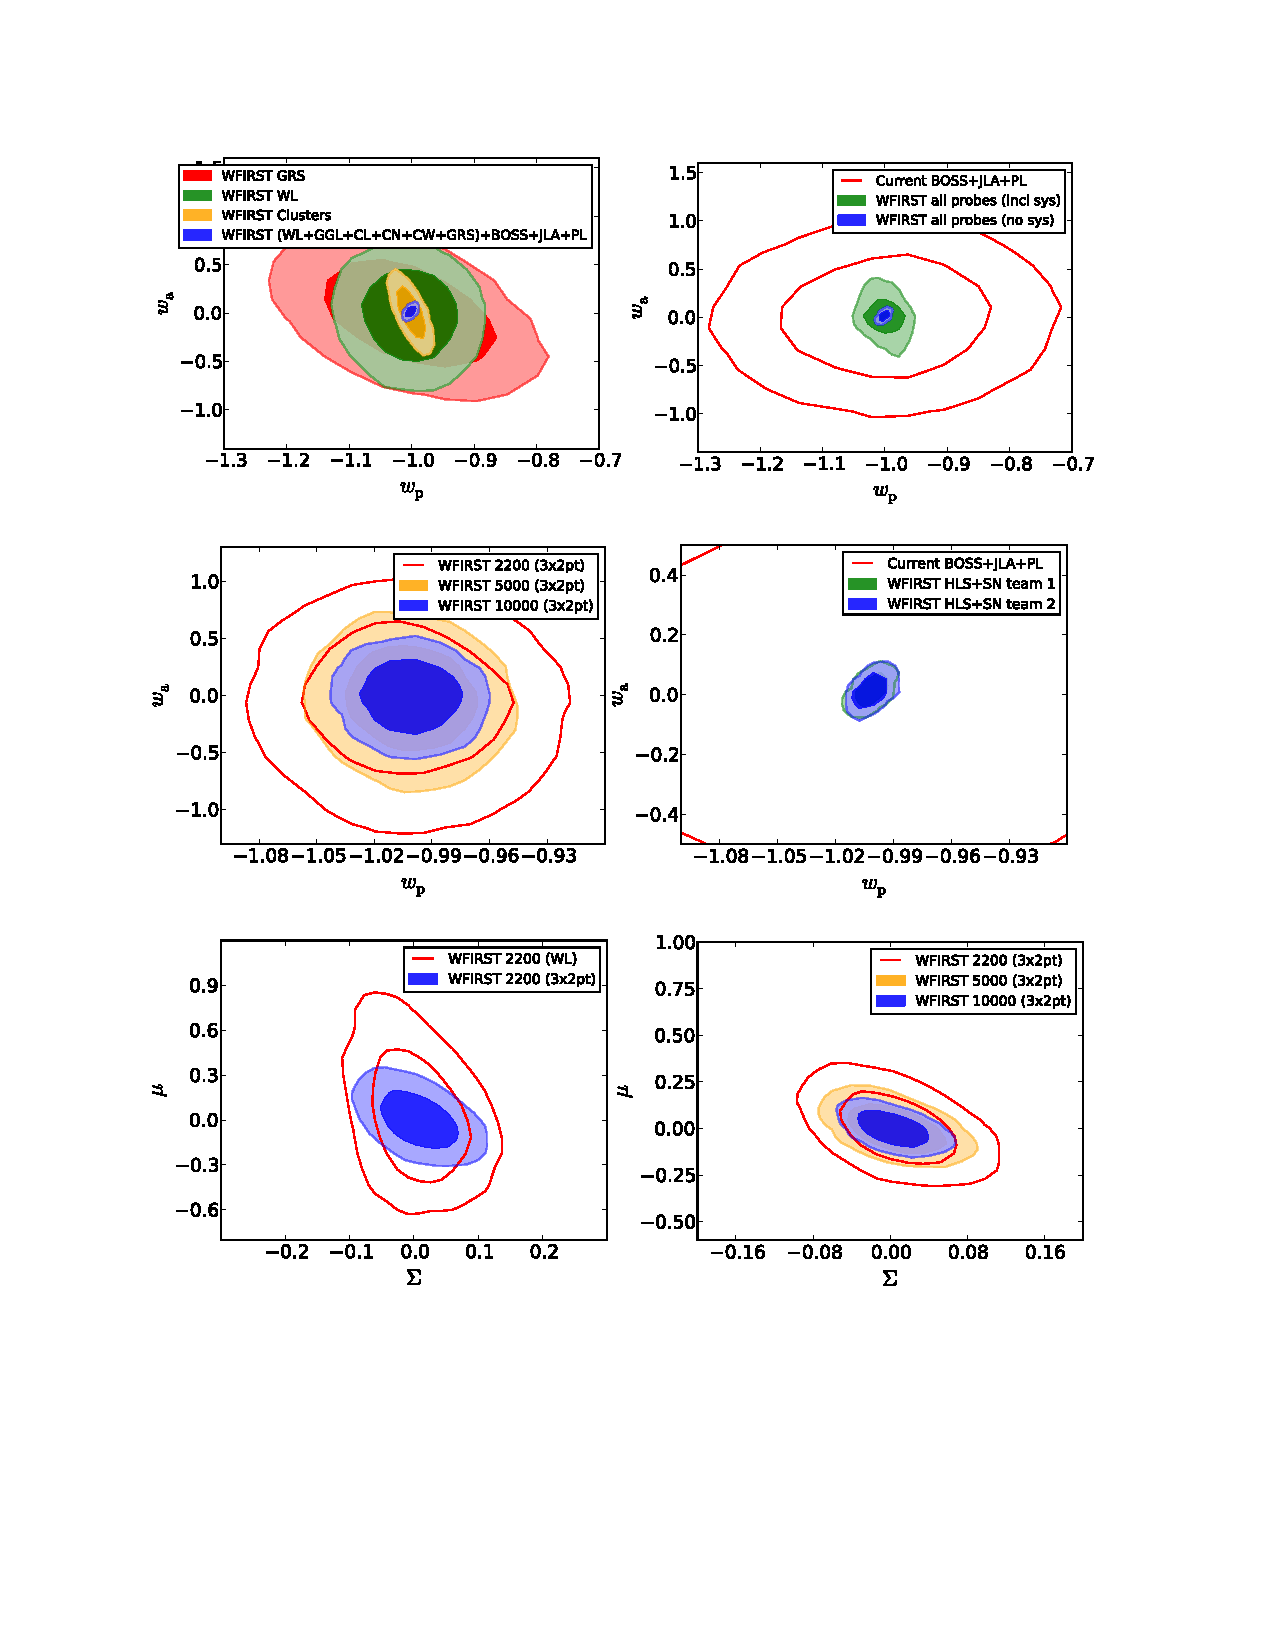
\includegraphics[width=15cm]{Plots/forecasts/multi}
\caption{WFIRST multi-probe studies, see text for details.}
\label{fi:multi}
\end{figure}

\subsubsection{\CoLi Multi-probe Analysis} Developing a multi-probe cosmology analysis framework is challenging given that the analysis pipeline for individual probes are each under continuous
development in order to meet the requirements of improving data quality. These
efforts have historically been largely independent from each other; as a
consequence, individual probe analyses utilize information from other probes to
offset/calibrate systematics. For example, one of the most important
astrophysical uncertainties for galaxy clustering is the relation of dark matter
halos and luminous galaxies. The joint analysis of clustering and galaxy-galaxy
lensing measurements removes uncertainties in this halo-galaxy connection when
constraining cosmology. However, cosmic shear analyses use the same
galaxy-galaxy lensing measurements to offset other systematic uncertainties
(e.g., intrinsic galaxy alignment). This is only one example of many systematics
mitigation conflicts that can occur when considering probes in isolation. A
multi-probe analysis framework must account for these correlated systematic
effects consistently across all probes; it cannot simply combine the optimal
versions of individual analyses and it must include a global, well-designed
systematics modeling and mitigation concept.

In this section we present a variety of simulated multi-probe WFIRST analyses.
Our results are summarized in Figure~\ref{fi:multi}. The upper left panel shows
the constraining power of the individual survey elements (galaxy-redshift
survey, weak lensing, galaxy clusters) in comparison to their combined
constraining power plus galaxy-galaxy lensing, photometric galaxy clustering,
and prior information from Planck, SN1a, BOSS\@. The likelihood analysis was
carried out in a 7-dimensional cosmological parameter space, excluding any
systematics. The right panel compares the aforementioned joint analysis (blue)
with the current state of the art (red) and we show how the contours increase
when including a realistic set of systematics in the analysis. These systematics
include uncertainties arising from shear and photo-$z$ calibration, cluster
mass-observable relation, galaxy intrinsic alignment, and galaxy bias. Modeling
and marginalizing over these systematics requires us to run a likelihood
analysis in 54 dimensional parameter space; the details of our analysis are very
similar to the LSST forecasts in~\citet{Krause2017}, but for WFIRST survey
parameters (survey area, number density, and redshift distribution).

The second row, left panel shows results from a simulated multi-probe analysis
that can be extracted from the imaging survey only. The so-called 3$\times$2pt analysis
consists of second-order statistics from weak lensing, photometric galaxy
clustering, and galaxy-galaxy lensing. We show the scaling of the error bars
(statistics only, no systematics) when going from the nominal survey area to a
5,000 and 10,000 deg$^2$ survey.

The second row, right panel shows again our full multi-probe analysis including
galaxy clusters and the spectroscopic survey component, i.e., BAO and RSD
measurements, and we also include information from the 2 WFIRST supernovae
teams. These team independently forecasted the WFIRST SN1a constraining power
and are in excellent agreement.

The lower row, left panel shows the constraining power of WFIRST weak lensing
and 3$\times$2pt for the nominal survey area on modified gravity parameters $\mu$ and
$\Sigma$ \citep[see e.g.,][for details]{jjk15, baa15}. The right panel shows the
constraining power when increasing the survey area again to 5,000 and 10,000
deg$^2$. The work on modified gravity extensions of \coli is led by JPL Postdocs Hironao Miyatake and Phil Bull in close collaboration with Tim Eifler and Elisabeth Krause and we plan to extend the results shown in Figure~\ref{fi:multi} to include further, recent developments in the field of modified gravity parameterization and classification. In particular, we plan to implement the ability to model modified gravity scenarios that belong to the class of Horndeski actions, which is the most general action for a single classical scalar field in the presence of gravity which does not result in any derivatives higher than second order in the equations of motion. 

We emphasize that multi-probe studies are an area of active research and that
the likelihood analyses presented here represents a first step towards our goal of optimally combining WFIRST internal observables and to study synergies between WFIRST and other, external data sets, in particular LSST\@.

\subsubsection{Other Signals in Multi-Probe Analysis} Spergel and his group have been exploring  the use of galaxy shapes to constrain primordial non-Gaussianity \citep{Chisari:2016xki}. Working with former Princeton student, Elisa Chisari, and former Princeton postdocs Cora Dvorkin and Fabian Schmidt, they showed that
multi-tracer weak lensing observations could create anisotropic non-Gaussianity. WFIRST
will be a powerful instrument for this approach.  Correlations between intrinsic
galaxy shapes on large-scales arise due to the effect of the tidal field of
large-scale structure. Anisotropic primordial non-Gaussianity induces a distinct
scale-dependent imprint in these tidal alignments on large scales. Motivated by
the observational finding that the alignment strength of luminous red galaxies
depends on how galaxy shapes are measured, we study the use of two different
shape estimators as a multi-tracer probe of intrinsic alignments. We show, by
means of a Fisher analysis, that this technique promises a significant
improvement on anisotropic non-Gaussianity constraints over a single-tracer
method. For future weak lensing surveys, the uncertainty in the anisotropic
non-Gaussianity parameter, $A_2$, is forecast to be $\sigma(A_2)\simeq 50$, $\sim$ 40\% smaller than
currently available constraints from the bispectrum of the Cosmic Microwave
Background. This corresponds to an improvement of a factor of 4−5 over the
uncertainty from a single-tracer analysis.

Emmanuel Schaan has been working with Spergel and with the JPL group to
explore the use of CMB  lensing measurements as a tool to calibrate
multiplicative bias \citep{Schaan:2016ois}.  WFIRST  will require exquisite control over systematic
effects. In their paper, they address shear calibration and present the most
realistic forecast to date for WFIRST and CMB lensing from a stage 4 CMB experiment
(CMB S4). We use the CosmoLike code to simulate a joint analysis of all the
two-point functions of galaxy density, galaxy shear and CMB lensing convergence.
We include the full Gaussian and non-Gaussian covariances and explore the
resulting joint likelihood with Monte Carlo Markov Chains. We constrain shear
calibration biases while simultaneously varying cosmological parameters, galaxy
biases and photometric redshift uncertainties. We find that CMB lensing from CMB
S4 enables the calibration of the shear biases down 0.6-3.2\% in 10 bins for
WFIRST (see Fig. \ref{fi:CMB}). For a given lensing survey, the method works best at high redshift where
shear calibration is otherwise most challenging. This self-calibration is robust
to Gaussian photometric redshift uncertainties and to a reasonable level of
intrinsic alignment. It is also robust to changes in the beam and the
effectiveness of the component separation of the CMB experiment, and slowly
dependent on its depth, making it possible with third generation CMB experiments
such as AdvACT and SPT-3G, as well as the Simons Observatory.


\begin{figure}
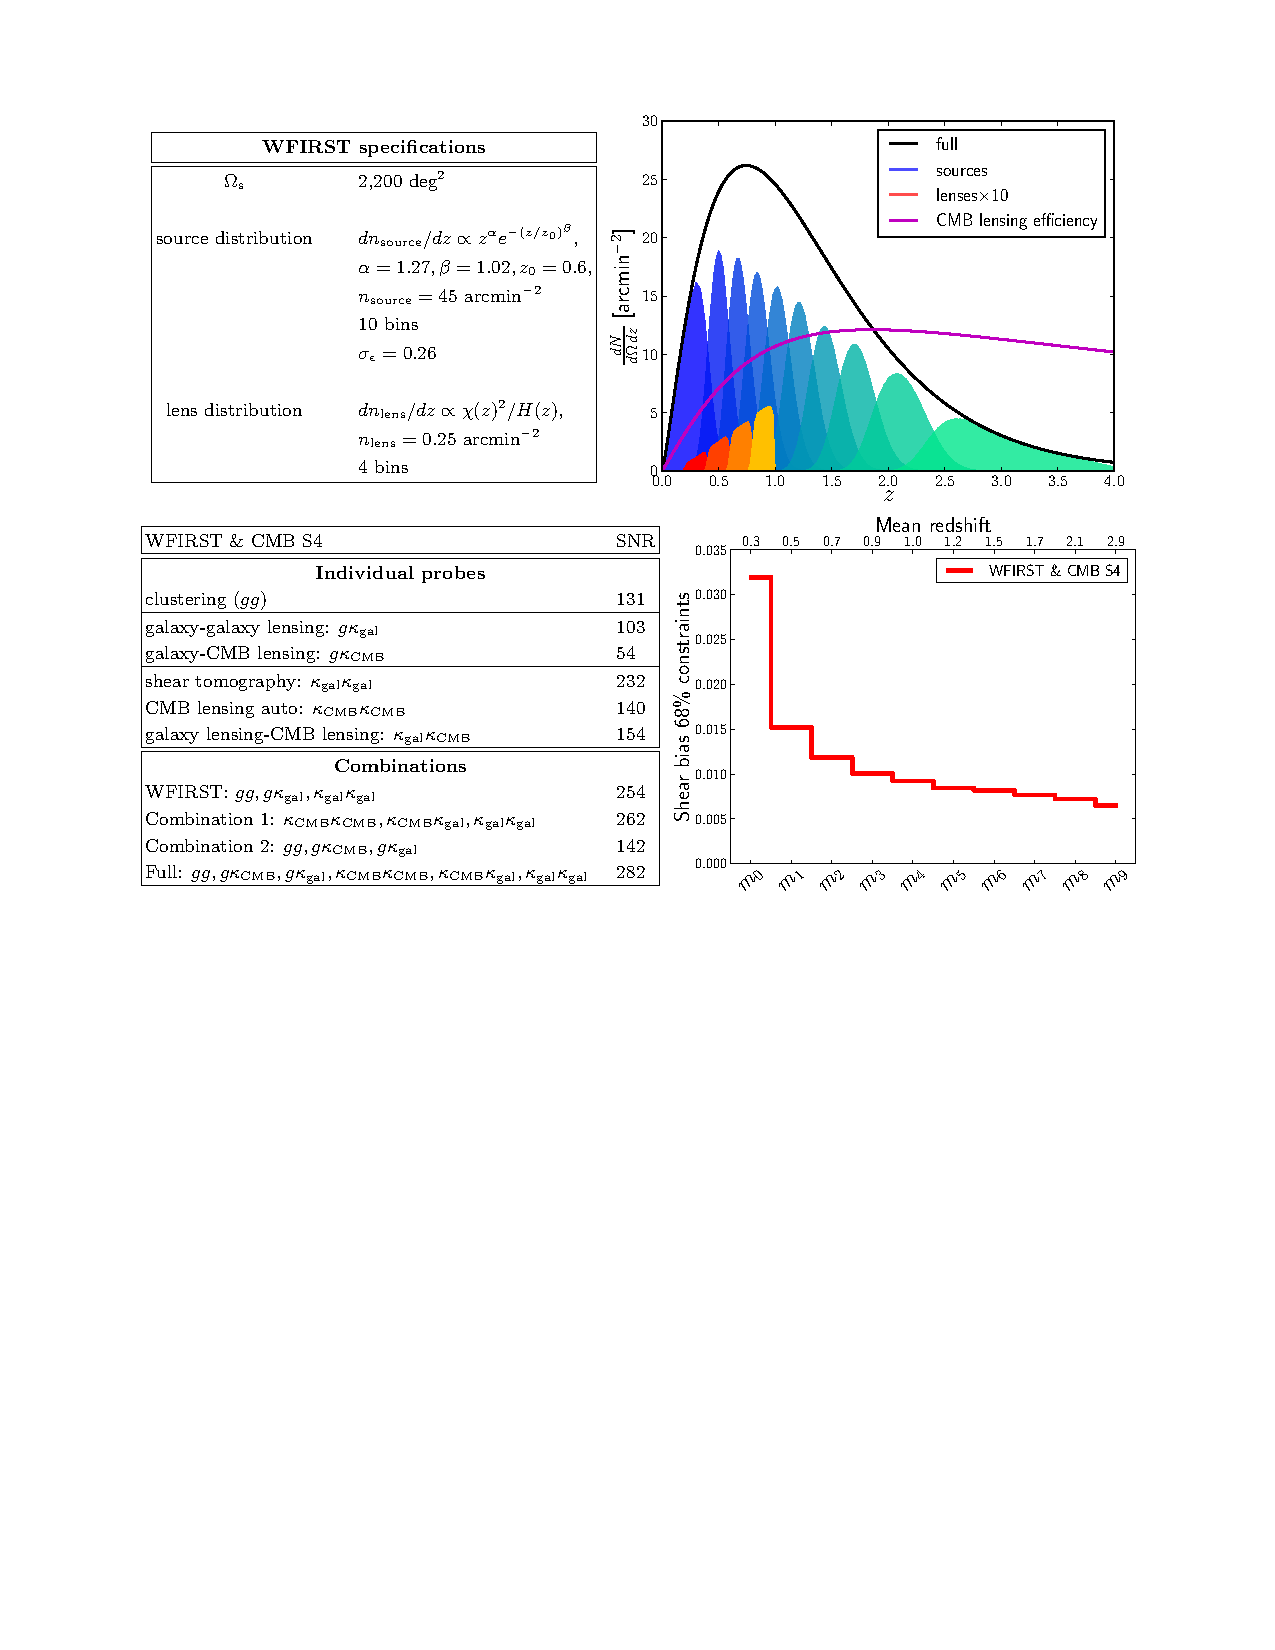
\includegraphics[width=15cm]{Plots/forecasts/CMB-S4-WFIRST}
\caption{Summary of the forecast for WFIRST and CMB S4 lensing. The top left panel summarizes our assumptions for
the WFIRST survey. The top right panel displays the photo-z bins assumed for the lens and source samples. The bottom left
panel summarizes the signal to noise ratios for the various probes and combinations. The bottom right panel shows the level
of shear calibration in WFIRST's ten source bins via CMB-S4 lensing. The calibration of the shear biases down 0.6-3.2\% in particular at high redshift bins, constitutes a promising alternative and an important cross-check to traditional simulation based approaches.}
\label{fi:CMB}
\end{figure}

\begin{summary}
Relying on our updates to the \CoLi package, we revised the cosmological
forecasts for the HLS spectroscopic and imaging survey. Using the unique \CoLi
capabilities, we conducted for the first time a full HLS multi-probe analysis in which we considered joint constraints between the HLS spectroscopic galaxy
sample, the HLS photometric galaxy samples, the HLS weak gravitational shear
signal, the HLS galaxy-galaxy lensing, the HLS galaxy clusters samples and the HLS SNe sample. Our
approach takes into account correlations between these probes as well as multiple systematic effects associated with each probe. We also combined WFIRST with other external surveys such as Planck and LSST. This is a milestone for our unified HLS SIT and we will investigate further the power and robustness of this multi-probe analysis in the coming years. We used this new capability to conduct trade studies to guide the development of the SRD. We also investigated new cosmological signals enabled by multi-probe studies, such as tests of general relativity.
\end{summary}
